\chapter{Bilinear and multilinear maps}
TODO: bilinear maps, bilinear forms = bilinear functionals
orthogonality

\section{Bilinear form}
\begin{definition}
Let $V$ be a vector space over a field $\F$. A function $B:V\times V\to \F$ is called a \udef{bilinear form} on $V$ if for all $v\in V$, both $B(v,-)$ and $B(-,v)$ are linear.
\end{definition}

\subsection{Quadratic forms}
\begin{definition}
Let $V$ be a vector space over a field $\F$ and $B$ a bilinear form on $V$. The function
\[ q_B: V\to \F: v\mapsto B(v,v) \]
is called the associated \udef{quadratic form}.
\end{definition}

\begin{proposition} \label{quadraticToBilinearForm}
Let $V$ be a vector space over a field $\F$ and $B$ a bilinear form on $V$. Then
\[ B(v,w) + B(w,v) = q_B(v+w) - q_B(v) - q_B(w). \]
\end{proposition}
\begin{corollary}
If $B$ is symmetric and $\F$ is not of characteristic $2$, then we can recover the bilinear form from the associated quadratic form:
\[ B(v,w) = \frac{1}{2}\Big(q_B(v+w) - q_B(v) - q_B(w)\Big). \]
\end{corollary}
So there is a bijection between symmetric and bilinear forms over fields not of characteristic $2$.

\begin{proposition}
Let $V$ be a vector space over a field $\F$ and $q: V\to \F$ a function. Then $q$ is the quadratic form associated to some bilinear form \textup{if and only if}
\begin{itemize}
    \item $\forall \lambda \in \F\forall v\in V: \; q(\lambda v) = \lambda^2 q(v)$;
    \item the parallelogram law holds: $\forall v,w\in V$
    \[ q(v+w) + q(v-w) = 2(q(v)+q(w)). \]
\end{itemize}
\end{proposition}
\begin{proof}
First assume $q$ is the quadratic form associated with the bilinear form $B$. Then $q(\lambda v) = B(\lambda v, \lambda v) = \lambda^2 B(v,v) = \lambda^2 q(v)$. The proof of the parallelogram law is the same as in an inner product space.

For the converse, we need to show that $q(v+w) - q(v) - q(w)$ is bilinear. TODO! (only real / complex??)
\end{proof}

\subsubsection{Finite dimensional quadratic forms}
TODO matrix representation of $q$.
\begin{definition}
Let $V$ be a finite dimensional vector space and $q$ a quadratic form on $V$. A basis $\{e_i\}_{i\in I}$ is called
\begin{itemize}
\item \udef{$q$-orthogonal} if $q(e_i + e_j) = q(e_i) + q(e_j)$ for all $i\neq j \in I$;
\item \udef{$q$-orthonormal} if it is orthogonal and $q(e_i)\in \{-1,0,1\}$ for all $i \in I$.
\end{itemize}
Let $\{e_i\}_{i\in I}$ be an orthonormal basis and
\begin{itemize}
    \item $p = |\setbuilder{e_i}{q(e_i) = 1}|$;
    \item $n = |\setbuilder{e_i}{q(e_i) = -1}|$;
    \item $z = |\setbuilder{e_i}{q(e_i) = 0}|$.
\end{itemize}
Then we call the triple $(p,n,z)$ the \udef{signature} of the basis $\{e_i\}_{i\in I}$.
\end{definition}

\begin{theorem}[Sylvester's law of inertia]
Let $V$ be a finite dimensional vector space and $q$ a quadratic form on $V$.
\begin{enumerate}
\item If $V$ is a real vector space, then any orthonormal basis has the same signature.
\item If $V$ is a complex vector space, then for any orthonormal basis, the pair $(p+n,z)$ is the same.
\end{enumerate}
\end{theorem}
\begin{proof}
TODO
\end{proof}

\begin{proposition}
Let $V$ be a finite dimensional vector space and $q$ a quadratic form on $V$.
\begin{enumerate}
\item If $\F$ is not of characteristic $2$, then $V$ has an orthogonal basis.
\item If $\F$ is a spin field, then $V$ has an orthonormal basis.
\end{enumerate}
\end{proposition}
TODO spin field.
\begin{proof}
TODO
\end{proof}


\section{Tensor product}
\url{https://kconrad.math.uconn.edu/blurbs/linmultialg/tensorprod.pdf}

\subsection{Abstract definition}
The idea behind the tensor product of two vector spaces $V,W$ over a field $K$ is to create the most general set of pairings that is a vector space and such that the pairings are bilinear: $\forall \lambda\in K: \forall v_1,v_2,v\in V:\forall w_1,w_2,w\in W$:
\[ (\lambda v_1+v_2, w) = \lambda (v_1,w)+(v_2,w) \qquad\text{and}\qquad (v,\lambda w_1+w_2) = \lambda (v,w_1) + (v,w_2). \]
This will be realised as a quotient of a free vector space.

To be more precise:
\begin{definition}
Let $V,W$ be vector spaces over a field $K$.
Consider the set $\operatorname{Field}(V)\times \operatorname{Field}(W)$, which we will refer to as $V\times W$. Construct the sets
\begin{align*}
R_1 &= \setbuilder{(\lambda(v_1,w)+(v_2,w),(\lambda v_1+v_2, w))\in F_K(V\times W)}{\lambda\in K; v_1,v_2\in V; w\in W} \\
R_2 &= \setbuilder{(\lambda(v,w_1)+(v,w_2),(v, \lambda w_1 + w_2))\in F_K(V\times W)}{\lambda\in K; v_1,v_2\in V; w\in W} \\
R &= R_1\cup R_2
\end{align*}
The \udef{tensor product} $V\otimes W$ of the vector spaces $V$ and $W$ is the quotient vector space
\[ V\otimes W := F(V\times W)/R^\equiv \]
where $R^\equiv$ is the reflexive symmetric transitive closure of $R$.

The equivalence class $[(v,w)]$ is denoted $v\otimes w$. An element of $V\otimes W$ that can be written as $v\otimes w$ is called a \udef{pure tensor} or \udef{simple tensor}.
\end{definition}
In order for the definition to be well-defined, we need for $R^\equiv$ to be a congruence on $F$.

The \udef{tensor product} $V\otimes W$ of two vector spaces $V$ and $W$ over a common field $K$ is the quotient vector space
\[ V\otimes W := F(V\times W)/\sim \]
where $\sim$ is the equivalence relation over the the free vector space $F(V\times W)$ with the properties of
\begin{itemize}
\item \textit{Distributivity}: $(v+v', w) \sim (v,w) + (v',w)$ and $(v, w+w') \sim (v,w) + (v,w')$.
\item \textit{Scalar multiples}: $c(v,w) \sim (cv,w) \sim (v,cw)$.
\end{itemize}



TODO definition via bases: $V\otimes W = F(\beta_V\times \beta_W)$

\begin{lemma} \label{tensorProductLinearlyIndependentBasis}
Let $V,W$ be vector spaces over a field $K$. Then
\[ V\otimes W = \setbuilder{\sum_{i=1}^n v_i\otimes w_i}{n\in \N, \text{$\{v_i\}_{i=1}^n\subseteq V$ and $\{w_i\}_{i=1}^n\subseteq W$ is a linearly independent}}. \]
\end{lemma}
\begin{proof}
Suppose $v_{j} = \sum_{k\neq j}\lambda_kv_k$. Then 
\[ \sum_{i=1}^n v_i\otimes w_i = \sum_{k\neq j}\lambda_kv_k\otimes w_k + \sum_{i\neq j} v_i\otimes w_i = \sum_{i\neq j}\lambda_iv_i\otimes w_i + \sum_{i\neq j} v_i\otimes w_i = \sum_{i\neq j} (\lambda_i+1)v_i\otimes w_i. \]
The argument for $\{w_i\}$ is similar.
\end{proof}

\subsection{Universal property}
See also proposition \ref{dimHomset}.


\subsection{Tensor product of linear maps}
The tensor product also operates on linear maps between vector spaces.
\begin{definition}
Given two linear maps $S: V\to X$ and $T:W\to Y$, then the \udef{tensor product} of the linear maps $S$ and $T$ is the linear map
\[ S\otimes T: V\otimes W \to X\otimes Y \]
defined by
\[ (S\otimes T)(v\otimes w) = S(v)\otimes T(w). \]
For vectors that are not pure tensors, this definition is extended by linearity.
\end{definition}
\begin{lemma}
The tensor product of linear maps is well-defined.
\end{lemma}

With this definition the tensor product becomes a bifunctor from the category of vector spaces to itself, covariant in both arguments.

TODO: functional calculus on tensor product.
TODO: tensor product of operator algebras


\subsection{Operator-valued matrices}
\begin{proposition}
Let $A$ be an algebra over a field $\mathbb{F}$ and $\beta$ any set. Consider the direct sum $A^\beta = \bigoplus_{i\in\beta}A$. Then $A^\beta \cong F_\F(\beta)\otimes A$.
\end{proposition}
\begin{proof}
TODO
\end{proof}


\subsection{Matrix representation}
\subsubsection{Finding a basis}
Assume $V$ and $W$ are finite-dimensional vector spaces with resp. bases $\{\vec{e}_i\}_i$ and $\{\vec{f}_j\}_j$. Then the set $\{ \vec{e}_i\otimes \vec{f}_j \}_{i,j}$ forms a basis for $V\otimes W$. Indeed,
\begin{itemize}
\item Take two arbitrary vectors $\vec{v} = \sum_i a_i \vec{e}_i \in V$ and $\vec{w} = \sum_j b_j \vec{f}_j \in W$.
Using the distributivity and scalar multiples properties of $\sim$, we can write the tensor product $\vec{v}\otimes \vec{w}$ as
\begin{equation} \vec{v}\otimes \vec{w} = (\sum_i a_i \vec{e}_i)\otimes(\sum_j b_j \vec{f}_j) = \sum_{i,j}a_ib_j (\vec{e_i}\otimes \vec{f}_j). \label{eq:vtensorw} \end{equation}
So any pure tensor can be written as the sum of vectors of the form $\vec{e}_i\otimes \vec{f}_j$. In general a vector in $V\otimes W$ can be written as a finite sum of pure tensors, meaning the set of vectors $\{ \vec{e}_i\otimes \vec{f}_j \}_{i,j}$ spans $V\otimes W$.
\item For linear independence we, observe that for any linearly independent $v_1, v_2, w_1, w_2$, the vector $v_1\otimes w_1 + v_2\otimes w_2$ cannot be written as a pure tensor.
\end{itemize}

Clearly it follows that
\[ \dim(V\otimes W) = \dim(V)\cdot\dim(W) \]

\subsubsection{Coordinates and the outer product}
The coordinates of a vector with respect to the basis $\{ \vec{e}_i\otimes \vec{f}_j \}_{i,j}$ can naturally be put into a matrix. Taking the tensor product of two vectors corresponds to taking the outer product of their coordinate vectors. That is, setting $\co(v) = \vec{v}$ and $\co(w) = \vec{w}$, we get
\[ \co(v\otimes w)_{i,j} = a_ib_j = (\vec{v}\vec{w}^\transp)_{i,j} \]
which follows from \eqref{eq:vtensorw} above.

For this reason $\otimes$ is also used to denote the outer product.

If we want a proper column vector as our coordinate vector, we can apply row-by-row vectorisation to this matrix.
\[ \co(v\otimes w) = \vectorisation_R(\vec{v}\vec{w}^\transp) = \vec{v}\otimes\vec{w} = \co(v)\otimes\co(w). \]
where $\otimes$ is also used to denote the Kronecker product.

Coordinates for vectors that are not pure tensors can easily be found by the linearity of the coordinate map.
\subsubsection{Linear maps and the Kronecker product}
Letting the coordinates be columns, we can hope to find a matrix for the linear map $S\otimes T$. Fix bases for the spaces $V,W,X,Y$. Let $A$ and $B$ be the matrices of $S$ and $T$ with respect to these bases. Use these bases to fix the bases for $V\otimes W$ and $X\otimes Y$.

\begin{eigenschap}
The matrix of the map $S\otimes T$ with respect to these bases is the matrix $A\otimes B$, where $\otimes$ is the Kronecker product.
\end{eigenschap}

This follows from a simple calculation:
\begin{align*}
\co\left(S\otimes T(v\otimes w)\right) &= \co\left(S(v)\otimes T(w)\right) \\
&= \co\left(S(v)\right)\otimes \co\left(T(w)\right) \\
&= A\co(v)\otimes B\co(v) \\
&= (A\otimes B)\co(v)\otimes\co(w) \qquad (\text{using the mixed product}) \\
&= (A\otimes B)\co(v\otimes w).
\end{align*}
Again this calculation can be extended to non-pure tensors by linearity.

\subsection{Properties}
TODO currying.
\url{https://math.stackexchange.com/questions/679584/why-is-texthomv-w-the-same-thing-as-v-otimes-w}
And reference later!
\subsection{Multilinear maps}
\begin{definition}
Let $V^k = V\times \ldots \times V$. A function $f: V^k\to \R$ is \udef{$k$-linear} if it is linear in each of its arguments.
\begin{itemize}
\item A $k$-linear function $f:V^k\to \R$ is \udef{symmetric} if for all permutations $\sigma\in S_k$
\[ f(v_{\sigma(1)},\ldots, v_{\sigma(k)}) = f(v_1,\ldots, v_k). \]
\item A $k$-linear function $f:V^k\to \R$ is \udef{alternating} if for all permutations $\sigma\in S_k$
\[ f(v_{\sigma(1)},\ldots, v_{\sigma(k)}) = (\sgn\sigma)f(v_1,\ldots, v_k). \]
\end{itemize}
We call the space of all alternating $k$-linear maps $A_k(V)$.
\end{definition}
In particular $A_1(V) = V^*$.
\begin{note}
Given a $k$-linear function $f$ and a permutation $\sigma\in S_k$, we define the $k$-linear function $\sigma f$ by
\[ (\sigma f)(v_1,\ldots, v_k) = f(v_{\sigma(1)},\ldots, v_{\sigma(k)}). \]
Then a symmetric map is one such that $\sigma f = f$ for all $\sigma\in S_k$ and an alternating map is one such that $\sigma f = (\sgn \sigma)f$ for all $\sigma\in S_k$.
\end{note} 
\begin{lemma}
Let $\sigma,\tau \in S_k$ and $f$ a $k$-linear map on $V$. Then $\tau(\sigma f) = (\tau \sigma)f$.
\end{lemma}
\subsubsection{The symmetrising and alternating maps}
\begin{definition}
Let $f$ be a $k$-linear map on a vector space $V$.
\begin{itemize}
\item The \udef{symmetrisation} of $f$, $Sf$, is the map
\[ Sf = \frac{1}{k!}\sum_{\sigma\in S_k}\sigma f. \]
\item The \udef{anti-symmetrisation} or \udef{skew-symmetrisation} of $f$, $Af$, is the map
\[ Af = \frac{1}{k!}\sum_{\sigma\in S_k}(\sgn \sigma)\sigma f. \]
\end{itemize}
\end{definition}
\begin{lemma}
\begin{enumerate}
\item The $k$-linear map $Sf$ is symmetric. If $f$ is symmetric, then $Sf = f$.
\item The $k$-linear map $Af$ is alternating. If $f$ is alternating, then $Af = f$.
\end{enumerate}
\end{lemma}
\begin{lemma} \label{idempotenceA}
Let $f$ be a $k$-linear functional and $g$ an $l$-linear functional on $V$. Then
\[ A(A(f)\otimes g) = A(f\otimes g) = A(f\otimes A(g)). \]
\end{lemma}
\subsubsection{The wedge product}
\begin{definition}
Let $f\in A_k(V)$ and $g\in A_l(V)$. The \udef{wedge product} of $f$ and $g$ is given by
\[ f\wedge g = \frac{(k+l)!}{k!l!}A(f\otimes g). \]
\end{definition}
We can also write
\[ (f\wedge g)(v_1,\ldots,v_{k+l}) = \frac{1}{k!l!}\sum_{\sigma\in S_{k+l}}(\sgn \sigma)f(v_{\sigma(1)},\ldots,v_{\sigma(k)})g(v_{\sigma(k+1)},\ldots, v_{\sigma(k+l)}). \]
We can reduce redundancies in this definition in the following way:
We call $\sigma\in S_{k+l}$ a \udef{$(k,l)$-shuffle} if
\[ \sigma(1)<\ldots<\sigma(k) \qquad \text{and}\qquad \sigma(k+1)<\ldots<\sigma(k+l). \]
The we write
\[ (f\wedge g)(v_1,\ldots,v_{k+l}) = \sum_{\text{$(k,l)$-shuffles $\sigma$}}(\sgn \sigma)f(v_{\sigma(1)},\ldots,v_{\sigma(k)})g(v_{\sigma(k+1)},\ldots, v_{\sigma(k+l)}). \]
\begin{proposition}
Let $f\in A_k(V)$ and $g\in A_l(V)$. Then
\[ f\wedge g = (-1)^{kl}g\wedge f. \]
\end{proposition}
\begin{lemma}
The wedge product is associative:
\[ (f\wedge g)\wedge h = f\wedge (g\wedge h). \]
\end{lemma}
Proof using \ref{idempotenceA}.

\begin{lemma}
Let $\alpha^1,\ldots, \alpha^k$ be linear functionals on $V$ and $v_1,\ldots,v_k\in V$, then
\[ (\alpha^1\wedge\alpha^k)(v_1,\ldots, v_k) = \det[\alpha^i(v_j)]. \]
\end{lemma}

\subsection{Tensors}
A $(p,k)$-tensor is a multilinear function $V^k\to V^p$.

\section{Real, complex and quaternionic vector spaces}
\begin{definition}
A function $f$ between complex vector spaces is \udef{anti-linear} (or \udef{conjugate-linear}) in the first component:
\[f(\lambda_1 v_1 + \lambda_2 v_2) = \overline{\lambda_1}f(v_1) + \overline{\lambda_2}f(v_2),\]
where $\lambda_1,\lambda_2 \in \C$ and $v_1,v_2\in \dom(f)$.
\end{definition}
\subsection{Complex structure on a real vector space}
\begin{definition}
Let $V$ be a real vector space. A \udef{complex structure} on $V$ is a linear map $J: V\to V$ such that $J^2 = -I_V$.
\end{definition}

\subsection{The real vector spaces associated to a complex vector space}
Let $V = (\C, V, +)$. Then define $V_\R \defeq (\R,V,+)$.

every anti-linear map $A:V\to W$ is an $\R$-linear map $A:V_\R\to W_\R$. (They are equal as sets).

\section{Quotient algebras of dual systems}
\begin{definition}
Let $\sSet{X,Y,b}$ be a dual system over a field $\F$. The algebra generated by this dual system is
\[ A(X,Y,b) \defeq \bigoplus_{n\in\N}(X\oplus Y)^{\otimes n}/\genIdealBuilder{x\otimes y - b(x,y)\vec{1}}{x\in X, y\in Y}. \]
\end{definition}
TODO universal algebra presented by generators and relation.

\subsection{The $\Z_2$-grading}
TODO parity grading grading respects ideal!

\begin{proposition}
Let $\sSet{X,Y,b}$ be a dual system. There is a faithfull superalgebra representation
\[ A(X,Y,b) \hookrightarrow \End\left(\bigoplus_{n\in \N}Y^{\otimes n}\right) \]
given by the extension (TODO universal property x2) of
\[ X\oplus Y \to \End(Y^{\otimes n}): x+y \mapsto \Big( y_1\otimes\ldots y_n \mapsto b(x,y_1) y\otimes y_2\otimes \ldots \otimes y_n \Big). \]
\end{proposition}

\section{Clifford algebras}
\begin{definition}
Let $V$ be a vector space over a field $\mathbb{F}$ and $q$ a quadratic form defined on $V$.
Let $\mathcal{T}(V)$ be the tensor algebra
\[ \mathcal{T}(V) \defeq \mathbb{F}\oplus \bigoplus_{n=1}^\infty V^n = \mathbb{F}\oplus \bigoplus_{n=1}^\infty \underbrace{V\otimes \ldots \otimes V}_{\text{$n$ times}}. \]
Let $\mathcal{I}(V,q)$ be the (two-sided) ideal in $\mathcal{T}(V)$ generated by
\[ \setbuilder{\vec{v}\otimes \vec{v} - q(v) \vec{1}}{\vec{v}\in V}. \]
Then the \udef{Clifford algebra} $\Cl(V,q)$ associated with $V$ and $q$ is the quotient
\[ \Cl(V,q) \defeq \mathcal{T}(V)/\mathcal{I}(V,q). \]
We call
\begin{itemize}
    \item elements of the Clifford algebra \udef{multivectors};
    \item elements of $\Span(V^k)$ \udef{$k$-vectors};
    \item elements of $V$ \udef{vectors}; we use bold face to denote these elements (e.g.\ $\vec{v}$);
    \item elements of $\F\vec{1}$ \udef{scalars}.
\end{itemize}
Elements of the Clifford algebra are called \udef{multivectors}.
\end{definition}
Let $\pi_q$ be the canonical projection
\[ \pi_q: \mathcal{T}(V) \to \Cl(V,q). \]


TODO: make all vectors bold!

\begin{lemma}
The embedding $V\hookrightarrow \Cl(V,q)$ is faithful, i.e.\ $\pi_q|_V$ is injective.
\end{lemma}
\begin{proof}
TODO
\end{proof}
Clearly $\pi_q|_V(\vec{v})^2 = q(\vec{v}) \vec{1}$ for all $\vec{v}\in V$.

\begin{lemma} \label{vectorInverseCliffordAlgebra}
Let $\Cl(V,q)$ be a Clifford algebra. Then
\[ \Cl^\times(V,q) \cap V = \setbuilder{\vec{v}\in V}{q(v) \neq 0}. \]
The inverse of $\vec{v}\in \Cl^\times(V,q) \cap V$ is $\vec{v}^{-1} = \vec{v}/q(\vec{v})$.
\end{lemma}
\begin{proof}
First take $\vec{v}\in \setbuilder{\vec{v}\in V}{q(\vec{v}) \neq 0}$. This definition of $\vec{v}^{-1}$ is indeed a multiplicative inverse: $\vec{v}\vec{v}^{-1} = \vec{v}^2/q(\vec{v}) = q(\vec{v})/q(\vec{v})\vec{1} = \vec{1}$.

Conversely, take $\vec{v}\in \Cl^\times(V,q) \cap V$. If $q(\vec{v}) = 0$, then $\vec{v}$ would be a zero divisor (as $\vec{v}\vec{v} = q(\vec{v})\vec{1} = 0$). No zero divisor can have an inverse (\ref{inverseZeroDivisor}), 
\end{proof}

\begin{lemma} \label{CliffordRelation}
The algebra $Cl(V,q)$ is generated by the vector space $V$ and $\vec{1}$, subject to the relations
\[ \vec{v}\vec{v} = q(\vec{v})\vec{1} \qquad \forall \vec{v}\in V. \]
\end{lemma}
TODO generators of an algebra!


Clifford algebras can also be defined by their universal property:
\begin{proposition}[Universal property of Clifford algebras] \label{CliffordUniversalProperty}
Let $V$ be a vector space over a field $\mathbb{F}$ and $q$ a quadratic form on $V$. 

Then for any unital associative algebra $A$ over $\mathbb{F}$ and linear map $j: V \to A$ such that
\[ j(\vec{v})^2 = q(\vec{v}) \vec{1} \qquad \forall \vec{v}\in V \]
there exists a unique algebra homomorphism $\widetilde{j}: \Cl(V,q)\to A$ such that the following diagram commutes:
\[ \begin{tikzcd}
V \rar{\pi_q|_V} \ar[dr, swap, "{j}"] & \Cl(V,q) \dar[dashed]{\widetilde{j}} \\
 & A
\end{tikzcd} \]
Furthermore, $\Cl(V,q)$ is the unique associative $\mathbb{F}$-algebra with this property.
\end{proposition}
\begin{corollary}
Let $(V,q)$ and $(V',q')$ be vector spaces with quadratic forms. If a linear map $f:V\to V'$ preserves to quadratic form, $q'\circ f = q$, then $f$ extends to a unique algebra homomorphism
\[ \widetilde{f}: \Cl(V,q) \to \Cl(V',q'). \]
Now let $(V^{\prime\prime},q^{\prime\prime})$ be another vector space equipped with a quadratic form and let $g: V'\to V^{\prime\prime}$ be a linear map preserving the quadratic form. Then
\[ \widetilde{g\circ f} = \widetilde{g}\circ\widetilde{f}. \]
Also isomorphisms of vector spaces extend to isomorphisms of Clifford algebras.
\end{corollary}
\begin{proof}
Let the algebra $A$ of the proposition be $\Cl(V',q')$. Then $\pi_q|_V\circ f$ satisfies the requirement for $j$:
\[ [(\pi_{q'}|_V\circ f)(\vec{v})]^2 = q'(f(\vec{v}))^2 \vec{1} = q(\vec{v})^2\vec{1}. \]
Thus by the proposition, there is a unique extension of $f:V\to V'$ to a map $\Cl(V,q) \to \Cl(V',q')$.

The composition relation follows from uniqueness.
\end{proof}
\begin{corollary} \label{qOrthogonalMaps}
The orthogonal group
\[ \Ogroup(V,q) = \setbuilder{g\in\GL(V)}{q\circ g = q} \]
extends canonically to a group of automorphisms of $\Cl(V,q)$:
\[ \Ogroup(V,q) \subset \Aut(\Cl(V,q)). \]
\end{corollary}

\subsection{Scalar and outer products}
\begin{lemma} \label{innerProductScalar}
Let $B: V\times V\to \F$ be a bilinear form on $V$ and consider the associated quadratic form $q: V\to\F : v\mapsto B(v,v)$.

For all $\vec{v},\vec{w}\in V\subseteq \Cl(V,q)$, we have $\vec{v}\vec{w} + \vec{w}\vec{v} = \big(B(v,w)+B(w,v)\big)\vec{1}$.
\end{lemma}
In particular, $\vec{v}\vec{w} + \vec{w}\vec{v}$ is a scalar multiple of the identity.
\begin{proof}
We can calculate
\[ q(\vec{v}+\vec{w})\vec{1} = (\vec{v}+\vec{w})^2 = \vec{v}^2 + \vec{v}\vec{w} + \vec{w}\vec{v} + \vec{w}^2 = \vec{v}\vec{w} + \vec{w}\vec{v} + q(\vec{v})\vec{1} + q(\vec{w})\vec{1}, \]
so $\vec{v}\vec{w}+\vec{w}\vec{v} = [q(\vec{v}+\vec{w})-q(\vec{v})-q(\vec{w})]\vec{1}$ and the result follows from \ref{quadraticToBilinearForm}.
\end{proof}

\begin{definition}
Let $\F$ be a field whose characteristic is not $2$ and $\Cl(V,q)$ a Clifford algebra over $\F$. We can then write, for $\vec{v},\vec{w}\in V$
\begin{align*}
\vec{v}\vec{w} &= \frac{\vec{v}\vec{w}+\vec{w}\vec{v}}{2} + \frac{\vec{v}\vec{w}-\vec{w}\vec{v}}{2} \\
&\defeq \vec{v}\cdot \vec{w} + \vec{v}\wedge \vec{w}.
\end{align*}
We call the symmetric part $\vec{v}\cdot \vec{w}$ the \udef{scalar product} (sometimes also called the \udef{inner product}),
and the antisymmetric part $\vec{v}\wedge \vec{w}$ the \udef{outer product}.
\end{definition}
If the quadratic form $q$ comes from a symmetric bilinear form $B$ (which is always the case of the characteristic of the field is not $2$), then $\vec{v}\cdot \vec{w} = B(v,w)\vec{1}$ by \ref{innerProductScalar}.

In the sequel, whenever we talk about the scalar and outer product, we will always assume the characteristic of the field is not $2$.

\begin{lemma}
Let $\Cl(V,q)$ be a Clifford algebra and $\vec{v}\in V$. Then $\vec{v}\cdot \vec{v} = q(\vec{v})\vec{1}$.
\end{lemma}

\begin{lemma}
Let $\Cl(V,q)$ be a Clifford algebra. Then the scalar and outer products are bilinear.
\end{lemma}
\begin{proof}
Take $a,b,c\in \Cl(V,q)$ and $\lambda \in \F$. Then
\[ (a + \lambda b)\cdot c = \frac{(a+\lambda b)c + c(a+\lambda b)}{2} = \frac{ac+\lambda bc + ca+\lambda cb}{2} = \frac{ac + ca}{2} + \lambda \frac{bc+ cb}{2} = a\cdot c + \lambda b\cdot c. \]
Linearity in the other argument follows from the symmetry of the scalar product. The argument for the outer product is analogous.
\end{proof}

\begin{lemma}
If we define the scalar and outer products as the (anti)-symmetrisation of general elements of the Clifford algebra, then for all $\vec{u}, \vec{v}, \vec{w}\in V$, we have
\begin{enumerate}
\item $(\vec{u}\cdot \vec{v})\cdot\vec{w} = \vec{u} \cdot (\vec{v}\cdot\vec{w})$;
\item $(\vec{u}\wedge \vec{v})\wedge\vec{w} = \vec{u} \wedge (\vec{v}\wedge\vec{w})$;
\end{enumerate}
\end{lemma}
TODO: this is not the right definition of these products.

TODO: generalise to more vectors.
\begin{proof}
We calculate
\[ (\vec{u}\cdot \vec{v})\cdot \vec{w} = \frac{\vec{u}\vec{v} +\vec{v}\vec{u}}{2}\cdot \vec{w} = \frac{1}{2}\big(\frac{\vec{u}\vec{v}\vec{w} + \vec{w}\vec{u}\vec{v}}{2} + \frac{\vec{v}\vec{u}\vec{w} + \vec{w}\vec{v}\vec{u}}{2}\big) = \frac{\vec{u}\vec{v}\vec{w} + \vec{w}\vec{u}\vec{v} + \vec{v}\vec{u}\vec{w} + \vec{w}\vec{v}\vec{u}}{4} = \frac{\vec{u}\vec{v}\vec{w} + \vec{w}\vec{u}\vec{v} + \vec{v}\vec{u}\vec{w} + \vec{w}\vec{v}\vec{u}}{4} \]
\end{proof}

\begin{lemma}
Let $\Cl(V,q)$ be a Clifford algebra and $\vec{v}\in V$. We have $\vec{v}\cdot \vec{v} = \vec{v}\vec{v} = \vec{v}^2 = q(\vec{v})\vec{1}$.
\end{lemma}
So $\vec{v}^2$ can cause no confusion.

\begin{lemma} \label{CliffordAlgebraVectorSwap}
Let $\Cl(V,q)$ be a Clifford algebra and $\vec{v},\vec{w}\in V$.
Then
\begin{enumerate}
\item $\vec{w}\vec{v} = 2(\vec{w}\cdot \vec{v}) - \vec{v}\vec{w}$;
\item $\vec{w}\vec{v} = 2(\vec{w}\wedge \vec{v}) + \vec{v}\vec{w} = -2(\vec{v}\wedge \vec{w}) + \vec{v}\vec{w}$;
\item $\vec{v}\vec{w}^2 = 2 (\vec{v}\cdot \vec{w})\vec{v}\vec{w} - \vec{v}^2 \vec{w}^2$;
\item $\vec{v}\vec{w}\vec{v} = 2(\vec{v}\cdot \vec{w})\vec{v} - q(\vec{v})\vec{w}$;
\item $\vec{v}^{-1}\vec{w}\vec{v} = 2\frac{\vec{v}\cdot \vec{w}}{q(\vec{v})}\vec{v} - \vec{w}$ if $\vec{v}$ is invertible;
\item $(\vec{v}\vec{u})^{-1}\vec{w}(\vec{v}\vec{u}) = \big(4 \frac{(\vec{u}\cdot \vec{v})(\vec{v}\cdot \vec{w})}{\vec{u}^2 \vec{v}^2} - 2 \frac{\vec{u}\cdot \vec{w}}{\vec{u}^2}\big)\vec{u} - 2 \frac{\vec{v}\cdot \vec{w}}{\vec{v}^2} \vec{v} + \vec{w}$ if $\vec{u}$ and $\vec{v}$ are invertible.
\end{enumerate}
\end{lemma}
\begin{proof}
(6) We calculate
\begin{align*}
(\vec{v}\vec{u})^{-1}\vec{w}(\vec{v}\vec{u}) &= \vec{u}^{-1}(\vec{v}^{-1}\vec{w}\vec{v})\vec{u} \\
&= \vec{u}^{-1}\big(2 \frac{\vec{v}\cdot \vec{w}}{\vec{v}^2}\vec{v} - \vec{w}\big)\vec{u} \\
&= 2 \frac{\vec{v}\cdot \vec{w}}{\vec{v}^2}\vec{u}^{-1}\vec{v}\vec{u} - \vec{u}^{-1}\vec{w}\vec{u} \\
&= 2 \frac{\vec{v}\cdot \vec{w}}{\vec{v}^2}\Big(2 \frac{\vec{u}\cdot \vec{v}}{\vec{u}^2}\vec{u} - \vec{v}\Big) - 2 \frac{\vec{u}\cdot \vec{w}}{\vec{u}^2}\vec{u} + \vec{w} \\
&= \Big(4 \frac{(\vec{u}\cdot \vec{v})(\vec{v}\cdot \vec{w})}{\vec{u}^2 \vec{v}^2} - 2 \frac{\vec{u}\cdot \vec{w}}{\vec{u}^2}\Big)\vec{u} - 2 \frac{\vec{v}\cdot \vec{w}}{\vec{v}^2} \vec{v} + \vec{w}.
\end{align*}
\end{proof}

\begin{lemma} \label{CliffordIdentities}
Let $\Cl(V,q)$ be a Clifford algebra and $\vec{v},\vec{w}\in V$.
Then
\begin{enumerate}
\item $\vec{v}(\vec{v}\wedge \vec{w}) = (\vec{w}\wedge \vec{v})\vec{v}$;
\item $(\vec{v}\wedge \vec{w})^{-1} = \frac{\vec{w}\wedge \vec{v}}{\vec{v}^2 \vec{w}^2 - (\vec{v}\cdot \vec{w})^2}$.
\end{enumerate}
\end{lemma}
\begin{proof}
(1) We calculate
\[ 2\vec{v}(\vec{v}\wedge \vec{w}) = q(\vec{v})\vec{w} - \vec{v}\vec{w}\vec{v} = \vec{w}q(\vec{v}) - \vec{v}\vec{w}\vec{v} = (\vec{w}\vec{v} - \vec{v}\vec{w})\vec{v} = 2(\vec{w}\wedge \vec{v})\vec{v}. \]

(2) We calculate
\begin{align*}
(\vec{v}\wedge \vec{w})(\vec{w}\wedge \vec{v}) &= \frac{1}{4}(\vec{v}\vec{w}- \vec{w}\vec{v})(\vec{w}\vec{v} - \vec{v}\vec{w}) \\
&= \frac{1}{4}\big(\vec{v}\vec{w}^2 \vec{v} + \vec{w}\vec{v}^2 \vec{w} - \vec{w}\vec{v}\vec{w}\vec{v} - \vec{v}\vec{w}\vec{v}\vec{w}\big) \\
&= \frac{1}{4}\Big(2\vec{v}^2\vec{w}^2 - \vec{w}\big(2(\vec{v}\cdot\vec{w}) - \vec{w}\vec{v}\big)\vec{v} - \vec{v}\big(2(\vec{v}\cdot\vec{w}) - \vec{v}\vec{w}\big)\vec{w}\Big) \\
&= \frac{1}{4}\Big(4\vec{v}^2\vec{w}^2 - 2(\vec{v}\cdot\vec{w})(\vec{v}\vec{w}+\vec{w}\vec{v})\Big) \\
&= \frac{1}{4}\Big(4\vec{v}^2\vec{w}^2 - 4(\vec{v}\cdot\vec{w})^2\Big) \\
&= \vec{v}^2\vec{w}^2 - (\vec{v}\cdot\vec{w})^2.
\end{align*}
\end{proof}

\subsubsection{Parallel and perpendicular vectors}
\begin{definition}
Let $\Cl(V,q)$ be a Clifford algebra. We call $\vec{v},\vec{w}\in V$
\begin{itemize}
\item \udef{orthogonal} or \udef{perpendicular} if $\vec{v}\cdot \vec{w} = 0$;
\item \udef{parallel} if $\vec{v}\wedge \vec{w} = 0$.
\end{itemize}
\end{definition}
\begin{lemma}
Let $\Cl(V,q)$ be a Clifford algebra and $\vec{v},\vec{w}\in V$. The following are equivalent:
\begin{enumerate}
\item $\vec{v}$ and $\vec{w}$ are orthogonal;
\item $\vec{v}\vec{w} = \vec{v}\wedge \vec{w}$;
\item $\vec{v}\vec{w} = -\vec{w}\vec{v}$;
\item $q(\vec{v}+\vec{w}) = q(\vec{v})+ q(\vec{w})$;
\end{enumerate}
as are
\begin{enumerate} \setcounter{enumi}{4}
\item $\vec{v}$ and $\vec{w}$ are parallel;
\item $\vec{v}\vec{w} = \vec{v}\cdot \vec{w}$.
\end{enumerate}
\end{lemma}

\begin{lemma}
Let $\Cl(V,q)$ be a Clifford algebra and $\vec{u},\vec{v}\in V$ be vectors. Then
\begin{enumerate}
\item $\vec{u} = (\vec{u}\cdot \vec{v})\vec{v}^{-1} + (\vec{u}\wedge \vec{v})\vec{v}^{-1}$;
\item $(\vec{u}\cdot \vec{v})\vec{v}^{-1}$ is parallel to $\vec{v}$ and $(\vec{u}\wedge \vec{v})\vec{v}^{-1}$ is perpendicular to $\vec{v}$.
\end{enumerate}
\end{lemma}
\begin{proof}
(1) We calculate
\[ \vec{u} = \vec{u}\vec{v}\vec{v}^{-1} = (\vec{u}\cdot \vec{v})\vec{v}^{-1} + (\vec{u}\wedge \vec{v})\vec{v}^{-1}. \]

(2) Since $(\vec{u}\cdot \vec{v})\vec{v}^{-1} = \frac{\vec{u}\cdot \vec{v}}{\vec{v}\cdot \vec{v}}\vec{v}$, it clearly commutes with $\vec{v}$.

We have that $(\vec{u}\wedge \vec{v})\vec{v}^{-1}$ anticommutes with $\vec{v}$ by \ref{CliffordIdentities}.
\end{proof}

\begin{definition}
Let $\Cl(V,q)$ be a Clifford algebra and $\vec{u},\vec{v}\in V$ be vectors. Then
\begin{itemize}
\item $\vec{u}_{\parallel \vec{v}} \defeq (\vec{u}\cdot \vec{v})\vec{v}^{-1}$ is the component of $\vec{u}$ parallel to $\vec{v}$;
\item $\vec{u}_{\perp \vec{v}} \defeq (\vec{u}\wedge \vec{v})\vec{v}^{-1}$ is the component of $\vec{u}$ perpendicular to $\vec{v}$.
\end{itemize}
\end{definition}

\begin{lemma} \label{parallelPerpendicularComponentConstructions}
Let $\Cl(V,q)$ be a Clifford algebra and $\vec{u},\vec{v}\in V$ be vectors. Then
\begin{enumerate}
\item $\vec{v}^{-1}\vec{u}\vec{v} = \vec{u}_{\parallel \vec{v}} - \vec{u}_{\perp \vec{v}}$;
\item $\vec{u}_{\parallel\vec{v}} = \frac{\vec{u}\cdot \vec{v}}{\vec{v}^2}\vec{v}$ and $\vec{u}_{\perp \vec{v}} = \vec{u} - \frac{\vec{u}\cdot \vec{v}}{\vec{v}^2}\vec{v}$;
\item $\vec{u}_{\perp \vec{v}}^2 = \vec{u}^2 - \frac{(\vec{u}\cdot \vec{v})^2}{\vec{v}^2} = \frac{\vec{u}^2 \vec{v}^2 - (\vec{u}\cdot \vec{v})^2}{\vec{v}^2}$;
\item $\vec{u}_{\perp \vec{v}}^{-1} = \frac{\vec{v}^2 \vec{u} - (\vec{u}\cdot\vec{v})\vec{v}}{\vec{u}^2 \vec{v}^2 - (\vec{u}\cdot \vec{v})^2}$.
\end{enumerate}
\end{lemma}
\begin{proof}
(1) We calculate
\begin{align*}
\vec{v}^{-1}\vec{u}\vec{v} &= \vec{v}^{-1}\big(\vec{u}_{\parallel \vec{v}} + \vec{u}_{\perp \vec{v}}\big)\vec{v} \\
&= \vec{v}^{-1}\vec{u}_{\parallel \vec{v}}\vec{v} + \vec{v}^{-1}\vec{u}_{\perp \vec{v}}\vec{v} \\
&= \vec{v}^{-1}\vec{v}\vec{u}_{\parallel \vec{v}} - \vec{v}^{-1}\vec{v}\vec{u}_{\perp \vec{v}} \\
&=\vec{u}_{\parallel \vec{v}} - \vec{u}_{\perp \vec{v}}.
\end{align*}

(2) Immediate.

(3) We calculate
\begin{align*}
\vec{u}_{\perp \vec{v}}^2 &= \big(\vec{u} - \frac{\vec{u}\cdot \vec{v}}{\vec{v}^2}\vec{v}\big)^2 \\
&= \vec{u}^2 + \frac{(\vec{u}\cdot \vec{v})^2\vec{v}^2}{\vec{v}^4} - \frac{\vec{u}\cdot \vec{v}}{\vec{v}^2}\vec{u}\vec{v} - \frac{\vec{u}\cdot \vec{v}}{\vec{v}^2}\vec{v}\vec{u} \\
&= \vec{u}^2 + \frac{(\vec{u}\cdot \vec{v})^2}{\vec{v}^2} - \frac{\vec{u}\cdot \vec{v}}{\vec{v}^2}(\vec{u}\vec{v} + \vec{v}\vec{u}) \\
&= \vec{u}^2 + \frac{(\vec{u}\cdot \vec{v})^2}{\vec{v}^2} - 2\frac{(\vec{u}\cdot \vec{v})^2}{\vec{v}^2} \\
&= \vec{u}^2 - \frac{(\vec{u}\cdot \vec{v})^2}{\vec{v}^2}.
\end{align*}

(4) We calculate
\begin{align*}
\vec{u}_{\perp \vec{v}}^{-1} &= \frac{\vec{u}_{\perp \vec{v}}}{\vec{u}_{\perp \vec{v}}^2} \\
&= \Big(\vec{u} - \frac{\vec{u}\cdot \vec{v}}{\vec{v}^2}\vec{v}\Big)\Big(\frac{\vec{v}^2}{\vec{u}^2 \vec{v}^2 - (\vec{u}\cdot \vec{v})^2}\Big) \\
&= \frac{\vec{v}^2 \vec{u} - (\vec{u}\cdot\vec{v})\vec{v}}{\vec{u}^2 \vec{v}^2 - (\vec{u}\cdot \vec{v})^2}.
\end{align*}
\end{proof}

\begin{definition}
Let $\Cl(V,q)$ be a Clifford algebra and $\vec{v}\in V$ a vector. Then the function $P_{\vec{v}}: V\to V: \vec{x}\mapsto \vec{v} + (\vec{x}\wedge \vec{v})\vec{v}^{-1}$ is the \udef{projection} onto the affine hyperplane determined by $\vec{v}$.
\end{definition}

\begin{lemma}
Let $\Cl(V,q)$ be a Clifford algebra and $\vec{v},\vec{x}\in V$ be vectors. Then $P_{\vec{v}}(\vec{x}) = \vec{v} + \frac{\vec{x} - \vec{v}^{-1}\vec{x}\vec{v}}{2}$.
\end{lemma}
\begin{proof}
We calculate
\[ P_{\vec{v}}(\vec{x}) = \vec{v} + (\vec{x}\wedge \vec{v})\vec{v}^{-1} = \vec{v} + \frac{1}{2}(\vec{x}\vec{v} - \vec{v}\vec{x})\vec{v}^{-1} = \vec{v} + \frac{\vec{x} - \vec{v}^{-1}\vec{x}\vec{v}}{2}. \]
\end{proof}

\subsection{Involutions}
\subsubsection{Grade involution}
Given a Clifford algebra $\Cl(V,q)$, consider the map $\alpha: V \to V: \vec{v}\mapsto -\vec{v}$ on the vector space $V$.
Now $\alpha$ is always an element of $\Ogroup(V,q)$, so by \ref{qOrthogonalMaps} it extends to a map on the Clifford algebra.
\[ \widetilde{\alpha}: \Cl(V,q) \to \Cl(V,q). \]
Since $\alpha^2 = I_V$, we have that
\[ \widetilde{\alpha}^2 = \widetilde{\alpha^2} = \widetilde{I_V} = I_{\Cl(V,q)} \]
meaning $\widetilde{\alpha}$ is an involution on the Clifford algebra. From now on we drop the tilde and just write $\alpha: \Cl(V,q) \to \Cl(V,q)$ for the \udef{grade involution}.

\begin{lemma}
The grade involution $\alpha: \Cl(V,q) \to \Cl(V,q)$
\begin{enumerate}
\item is an algebra homomorphism and thus multiplicative:
\[ \alpha(xy) = \alpha(x)\alpha(y) \qquad\forall x,y\in \Cl(V,q); \]
\item is unital, $\alpha(\vec{1}) = \vec{1}$, and thus preserves inverses:
\[ \alpha(x^{-1}) = \alpha(x)^{-1} \qquad\forall x\in \Cl(V,q); \]
\item generates a $\Z_2$-grading 
\[ \Cl(V,q) = \Cl^0(V,q)\oplus \Cl^1(V,q). \]
\end{enumerate}
\end{lemma}

\subsubsection{Transpose}
The transpose map defined on the tensor algebra $\mathcal{T}(V)$, i.e.\ the linear map that reverses to order of homogeneous elements:
\[ v_1\otimes \ldots \otimes v_r \mapsto v_r \otimes \ldots \otimes v_1, \]
preserves the ideal $\mathcal{I}(V,q)$, and so determines a well-defined map on the Clifford algebra $\Cl(V,q)$:
\[ (-)^t: \Cl(V,q)\to \Cl(V,q). \]
\begin{lemma}
The transpose $(-)^t: \Cl(V,q)\to \Cl(V,q)$ is
\begin{enumerate}
\item an involution;
\item an anti-automorphism:
\[ \forall x,y\in \Cl(V,q): \quad (xy)^t = y^tx^t; \]
\item unital.
\end{enumerate}
\end{lemma}

\subsubsection{Clifford conjugation}
\begin{definition}
The composition of the grade involution and the transpose is called \udef{Clifford conjugation}:
\[ x\mapsto \overline{x} \defeq \alpha(x^t). \]
\end{definition}
\begin{lemma}
The grade involution and transpose commute
\[ \alpha \circ(-)^t = (-)^t\circ \alpha \]
and Clifford conjugation is thus equal to both.
\end{lemma}

\begin{lemma}
Clifford conjugation is
\begin{enumerate}
\item an involution;
\item an anti-automorphism:
\[ \forall x,y\in \Cl(V,q): \quad (xy)^t = y^tx^t; \]
\item unital.
\end{enumerate}
\end{lemma}

\subsubsection{Quaternion types of Clifford algebra types}

\subsection{The norm mapping}
\begin{definition}
We define the \udef{norm mapping} $N$ by
\[ N: \Cl(V,q)\to \Cl(V,q): x\mapsto x \overline{x}. \]
\end{definition}
\begin{lemma} \label{normIsQuadraticForm}
\begin{enumerate}
\item If $v\in V$, then $N(v) = q(v)$.
\item $\alpha\circ N = N\circ \alpha$.
\end{enumerate}
\end{lemma}

\begin{proposition}
Let $\Cl(V,q)$ be a Clifford algebra and $\vec{v},\vec{w}\in V$. Then
\begin{enumerate}
\item $N(\vec{v}\vec{w}) = \vec{v}^2 \vec{w}^2$;
\item $N(\vec{v}\wedge \vec{w}) = \vec{v}^2\vec{w}^2 - (\vec{v}\cdot \vec{w})^2$;
\end{enumerate}
\end{proposition}
\begin{proof}
(1) Because $\vec{v}\vec{w}\in\Cl(V,q)^0$, we have $N(\vec{v}\vec{w}) = (\vec{v}\vec{w})(\vec{w}\vec{v}) = \vec{v}^2 \vec{w}^2$.

(2) Because $\vec{v}\wedge \vec{w}\in\Cl(V,q)^0$, we have $N(\vec{v}\wedge \vec{w}) = (\vec{v}\wedge \vec{w})(\vec{w}\wedge \vec{v})$. We use $\vec{v}\wedge \vec{w} = -\vec{w}\wedge \vec{v} = \vec{v}\vec{w} - \vec{v}\cdot \vec{w}$ to calculate
\[ N(\vec{v}\wedge \vec{w}) = -(\vec{v}\vec{w} - \vec{v}\cdot \vec{w})(\vec{v}\vec{w} - \vec{v}\cdot \vec{w}) = -\vec{v}\vec{w}\vec{v}\vec{w} + 2(\vec{v}\cdot \vec{w})\vec{v}\vec{w} - (\vec{v}\cdot\vec{w})^2 \]
Then \ref{CliffordAlgebraVectorSwap} gives $\vec{v}\vec{w}\vec{v}\vec{w} = 2 (\vec{v}\cdot \vec{w})\vec{v}\vec{w} - \vec{v}^2 \vec{w}^2$.
Plugging this back in gives
\[ N(\vec{v}\wedge \vec{w}) = -2 (\vec{v}\cdot \vec{w})\vec{v}\vec{w} + \vec{v}^2 \vec{w}^2 + 2(\vec{v}\cdot \vec{w})\vec{v}\vec{w} - (\vec{v}\cdot\vec{w})^2 = \vec{v}^2 \vec{w}^2 - (\vec{v}\cdot\vec{w})^2. \]
\end{proof}


\subsection{Clifford algebras as filtered algebras}
\begin{proposition}
A Clifford algebra $\Cl(V,q)$ has a filtration $F_k \defeq \Span(V^{k})$.
\end{proposition}

We then have an associated graded algebra and a grade operator.

\begin{proposition}
Let $V$ be a vector space and $q$ a quadratic form on $V$.
\begin{enumerate}
\item As graded algebras, $\Cl(V,q)$ is naturally isomorphic to the exterior algebra ${\textstyle\bigwedge}^* V$.
\item As algebras ${\textstyle\bigwedge}^* V \cong \Cl(V,0)$.
\item As vector spaces, there is an isomorphism
\[ {\textstyle\bigwedge}^* V \to \Cl(V,q): v_1\wedge \ldots \wedge v_n \mapsto \frac{1}{r!}\sum_{\sigma\in S_n}\sgn(\sigma)v_{\sigma(1)}\hdots v_{\sigma(r)} \]
compatible with the fibrations.
\end{enumerate}
\end{proposition}

\begin{lemma}
Let $\Cl(V,q)$ be a Clifford algebra and $\vec{v},\vec{w}\in V$. Then $\grade{\vec{v}\vec{w}}_1 = 0$.
\end{lemma}
\begin{proof}
We have $\alpha(\vec{v}\vec{w}) = (-\vec{v})(-\vec{w}) = \vec{v}\vec{w}$, so $\vec{v}\vec{w}\in\Cl^0(V,q)$, while $V\subseteq \Cl^1(V,q)$.
\end{proof}

\begin{proposition}
Let $\Cl(V,q)$ be a Clifford algebra and $\vec{v}_1, \ldots, \vec{v}_k\in V$. Then $\vec{v}_1\ldots\vec{v}_k \in V^{k-1}$ \textup{if and only if} $\vec{v}_1,\ldots,\vec{v}_k$ are linearly dependent.
\end{proposition}
\begin{proof}
If $\vec{v}_1, \ldots, \vec{v}_k\in V$ are linearly dependent, then we can eliminate one of the $\vec{v}_j$ and then $\vec{v}_1\ldots\vec{v}_k \in V^{k-1}$.

Now assume $\vec{v}_1, \ldots, \vec{v}_k\in V$ are linearly independent.
\end{proof}

\subsection{Orthogonal decomposition}
As $q(u,v)$ is a bilinear form, we can consider orthogonal subspaces with respect to it. Then $V=V_1\oplus V_2$ is a $q$-orthogonal decomposition if and only if $\forall v_1\in V_1, v_2\in V_2$:
\[ q(v_1,v_2) = 0 \qquad \iff \qquad q(v_1+v_2) = q(v_1) + q(v_2). \]
\begin{proposition}
Let $V=V_1\oplus V_2$ be a $q$-orthogonal decomposition. Then there is a natural isomorphism of Clifford algebras
\[ \Cl(V,q) \;\to\; \Cl(V_1,q|_{V_1}) \hat{\otimes} \Cl(V_2, q|_{V_2}):\quad v_1+v_2\mapsto v_1\otimes \vec{1} + \vec{1}\otimes v_2. \]
\end{proposition}

\section{Subgroups of a Clifford algebra}

\begin{proposition}
Let $V$ be a finite-dimensional real or complex vector space of dimension $\dim V = n$. Then the group $\Cl^\times(V,q)$ of multiplicative units in the Clifford algebra is a Lie group of dimension $2^n$ and the corresponding Lie algebra $\mathfrak{cl}^\times(V,q)$ is the full Clifford algebra $\Cl(V,q)$ with the Lie bracket
\[ [x,y] = xy - yx.  \]
\end{proposition}

\subsection{Inner automorphisms of $\Cl(V,q)$}
Characteristic for field not 2!!

\begin{lemma}
Let $\vec{v}\in V\setminus\{0\}$. Then $\Ad_{\vec{v}} = \Ad_{\vec{v}^{-1}}$.
\end{lemma}
\begin{proof}
For all $x\in Cl(V,q)$, we have
\[ \Ad_{\vec{v}}(x) = \vec{v}^{-1}x\vec{v} = \frac{\vec{v}x\vec{v}}{q(\vec{v})} = \vec{v}x\vec{v}^{-1} = \Ad_{\vec{v}^{-1}}(x). \]
\end{proof}

\begin{proposition} \label{AdOrthogonalDecomposition}
Let $\vec{v}\in V\cap \Cl^\times(V,q)$. Then for all $\vec{w}\in V$:
\[ \Ad_{\vec{v}}(\vec{w}) = \frac{\vec{v}\vec{w}\vec{v}}{q(\vec{v})} = \frac{2\vec{v}\cdot\vec{w}}{q(\vec{v})}\vec{v} - \vec{w}. \]
In particular $\Ad_{\vec{v}}[V] = V$.
\end{proposition}
\begin{proof}
From \ref{vectorInverseCliffordAlgebra} we have $q(\vec{v})\neq 0$ and $\vec{v}^{-1} = \vec{v}/q(\vec{v})$.
We then calculate
\[ q(\vec{v})\Ad_{\vec{v}}(\vec{w}) = q(\vec{v})\vec{v}\vec{w}\vec{v}^{-1} = \vec{v}\vec{w}\vec{v} = (\vec{v}\vec{w} + \vec{w}\vec{v} - \vec{w}\vec{v})\vec{v} = (\vec{v}\vec{w}+\vec{w}\vec{v})\vec{v} - q(\vec{v})\vec{w}. \]
\end{proof}

\begin{lemma} \label{AdOrthogonalMap}
Let $\vec{v}\in V$ such that $q(\vec{v})\neq 0$. Then $\Ad_{\vec{v}}\in \Ogroup(V,q)$.
\end{lemma}
TODO renew notation
\begin{proof}
Clearly $\Ad_{\vec{v}}$ is invertible. We then calculate using \ref{AdOrthogonalDecomposition}
\begin{align*}
q(\Ad_v(w)) &= q\left(\frac{q(v,w)}{q(v)}v - w\right) = q\left(\frac{q(v,w)}{q(v)}v,-w\right) + q\left(\frac{q(v,w)}{q(v)}v\right) + q(w) \\
&= -\frac{q(v,w)}{q(v)}q(v,w)+\left(\frac{q(v,w)}{q(v)}\right)^2q(v) + q(w) = q(w).
\end{align*}
\end{proof}


\subsection{Pin and Spin groups}
\begin{definition}
Let $P(V,q)$ be the subgroup of $\Cl^\times(V,q)$ generated by elements $v\in V$ with $q(v)\neq 0$.

We also define the group
\[ \Gamma(V,q) \defeq \setbuilder{x\in\Cl^\times(V,q)}{\Ad_x[V] = V}. \]
which is called the \udef{Clifford group}, \udef{Lipschitz group} or \udef{Clifford-Lipschitz group}.
\end{definition}
That $\Gamma(V,q)$ is a group follows from the following observation: If $\Ad_x[V]=V$ and $\Ad_y[V]=V$, then
\[ \Ad_{xy}[V] = \Ad_x[\Ad_y[V]] = \Ad_x[V] = V. \]


\begin{lemma} \label{PsubgroupVpreserving}
There is an inclusion
\[ P(V,q) \subset \Gamma(V,q). \]
\end{lemma}
\begin{proof}
The generators of $P(V,q)$ are in $\Gamma(V,q)$ by \ref{AdOrthogonalDecomposition} and $\Gamma(V,q)$ is a group.
\end{proof}

\begin{lemma}
The $\Ad$ function defines a representation
\[ \Ad: P(V,q) \to \Ogroup(V,q). \]
\end{lemma}
\begin{proof}
This mapping is well-defined by \ref{AdOrthogonalMap} and the identity
\[ \Ad_{xy} = \Ad_x\circ \Ad_y. \]
This identity also shows that the mapping is a group homomorphism, and thus that it is a representation.
\end{proof}

\begin{lemma}
Let $x\in \Gamma(V,q)$. Then
\begin{enumerate}
\item $\alpha(x)\in \Gamma(V,q)$;
\item $x^t\in \Gamma(V,q)$.
\end{enumerate}
\end{lemma}
\begin{proof}
We calculate
\[ V = \alpha[V] = \alpha[\Gamma(V,q)] = \alpha(\alpha(x)) V \alpha(x)^{-1} = \Ad_{\alpha(x)}[V] \]
and
\[ V = (\alpha[V])^t = \alpha(x^t) V (x^t)^{-1} = \Ad_{x^t}[V] \]
and the third follows by multiplicative closure.
\end{proof}
A consequence of this lemma is that $N(x)\in \Gamma(V,q)$ for all $x\in \Gamma(V,q)$. But we will show that something stronger holds, namely $N(x)\in\F^\times$.

\begin{definition}
The \udef{Pin group} of $(V,q)$ is the subgroup $\Pin(V,q)$ of $P(V,q)$ generated by the elements $v\in V$ with $q(v) = \pm 1$.

The \udef{Spin group} of $(V,q)$ is defined by
\[ \Spin(V,q) = \Pin(V,q) \cap \Cl^0(V,q) \]
where $\Cl^0(V,q)$ is the even subalgebra of $\Cl(V,q)$.
\end{definition}

\subsection{The twisted adjoint representation}
Consider the map $\Ad_v$ acting on the $q$-orthogonal decomposition (TODO ref)
\[ V = \Span\{v\}\oplus\Span\{v\}^\perp \qquad \text{for some $v\in P(V,q)$,} \]
where $\Span\{v\}^\perp = \setbuilder{w\in V}{q(v,w)=0}$. Then, by the formula
\[ \Ad_v(w) = \frac{q(v,w)}{q(v)}v - w ,\]
we see that elements of $\Span\{v\}$ are mapped to themselves:
\begin{align*}
\Ad_v(\lambda v) &= \frac{q(v,\lambda v)}{q(v)}v - \lambda v = \lambda\frac{q(2v)-2q(v)}{q(v)}v - \lambda v \\
&= 2\lambda v -\lambda v = \lambda v.
\end{align*}
and that elements $w\in\Span\{v\}^\perp$ are mapped to $-w$.

This means that $\Ad_v$ is orientation-preserving if $\dim(V)$ is odd and orientation-reversing otherwise.

We would prefer the action of $\Ad_v$ to do the opposite: fix the hyperplane $\Span\{v\}^\perp$ and invert $\Span\{v\}$. To that end we introduce the twisted adjoint representation.
\begin{definition}
The \udef{twisted adjoint representation} $\widetilde{\Ad}: \Cl^\times(V,q) \to \GL(\Cl(V,q))$ is defined by
\[ \widetilde{\Ad}_x(y) = \alpha(x)yx^{-1} \qquad \forall x\in \Cl^\times(V,q), \forall y\in \Cl(V,q) \]
where $\alpha$ is the grade involution.
\end{definition}
\begin{lemma}
Let $x,y\in \Cl^\times(V,q)$ and $v,w\in V$. Then
\begin{enumerate}
\item $\widetilde{\Ad}_{xy} = \widetilde{\Ad}_x\circ \widetilde{\Ad}_y$;
\item $\widetilde{\Ad}_x = \Ad_x$ if $x\in \Cl^0(V,q)$;
\item $\widetilde{\Ad}_v(w) = w-\frac{q(v,w)}{q(v)}v$.
\end{enumerate}
\end{lemma}

We have
\[ \Gamma(V,q) = \setbuilder{x\in\Cl^\times(V,q)}{\widetilde{\Ad}_x[V] = V}. \]

\begin{proposition}
Let $V$ be a finite-dimensional vector space over a field $\mathbb{F}$ and $q$ non-degenerate. Then the kernel of the homomorphism
\[ \widetilde{\Ad}: \Gamma(V,q) \to \GL(V) \]
is exactly the group $\mathbb{F}^\times$.
\end{proposition}
\begin{proof}
Choose an orthogonal basis $v_1,\ldots, v_n$ for $V$ w.r.t. the bilinear form $q(-,-)$ (TODO ref; also proof here only finite-dim: can it generalise?). Suppose $x\in \Cl^\times(V,q)$ is in the kernel of $\widetilde{\Ad}$, then
\[ \alpha(x)v = vx \qquad \text{for all $v\in V$.} \]
Now we can write $x = x_0 + x_1$ where $x_0$ is even and $x_1$ is odd and both are polynomial expressions in $v_1,\ldots, v_n$. Making use of $v_iv_j = \pm v_jv_i$, we can write $x_0 = a_0 + v_1a_1$ where $a_0,a_1$ are polynomial expressions in $v_2,\ldots, v_n$. Then $a_0$ is even and $a_1$ is odd, so
\[ v_1a_0 + v_1^2a_1 = v_1(a_0+v_1a_1) = (a_0+v_1a_1)v_1 = a_0v_1 + v_1 a_1 v_1 = v_1a_0-v_1^2 a_1. \]
Thus $v^2_1a_1 = -q(v_1)a_1 = 0$, so $a_1=0$ and $x_0$ does not involve $v_1$. By induction $x_0$ does not involve any of $v_1,\ldots, v_n$ and thus $x_0 = \lambda \vec{1}$ for $\lambda\in\mathbb{F}$.

A similar argument shows that $x_1$ is independent of $v_1,\ldots, v_n$ and thus $x_1=0$. Here it is important that $v_1x_1 = -x_1v_1$, because in $x_1 = a_0 + v_1a_1$, $a_0$ is now odd and $a_1$ even.

Thus $x = x_0+x_1 = \lambda \vec{1}$ and $x\neq 0$, so $x\in \mathbb{F}^\times$.
\end{proof}
This proof only works for the \textit{twisted} adjoint representation, not the adjoint representation.

It is also clearly important that $q$ be non-degenerate.

\begin{corollary} \label{normHomomorphism}
The restriction of the norm $N$ to $\Gamma(V,q)$ gives a homomorphism
\[ N: \Gamma(V,q) \to \mathbb{F}^\times. \]
\end{corollary}
\begin{proof}
If we can show that $N[\Gamma(V,q)]\subset \mathbb{F}^\times$, then the multiplicativity of $N$ follows from
\[ N(xy) = xy\alpha((xy)^t) = xy\alpha(y^t)\alpha(x^t) = xN(y)\alpha(x^t) = x\alpha(x^t)N(y) = N(x)N(y). \]

Thus by the proposition it is enough to show that for all $x\in \Gamma(V,q)$, $N(x)\in \ker(\widetilde{\Ad})$. Because $\alpha(x)vx^{-1}\in V$, the transpose leaves it unchanged:
\[ \alpha(x)vx^{-1} = (\alpha(x)vx^{-1})^t = (x^t)^{-1}v\alpha(x^t). \]
This can be rewritten as
\[ v = x^t\alpha(x)vx^{-1}(\alpha(x^t))^{-1} = \alpha(\alpha(x^t)x)v(\alpha(x^t)x)^{-1} = \widetilde{\Ad}_{N(x)}(v). \]
Thus $N(x)\in \ker(\widetilde{\Ad})$.
\end{proof}
\begin{corollary}
Let $x\in \Gamma(V,q)$, then $\widetilde{\Ad}_x \in \Ogroup(V,q)$. Thus there is a group homomorphism
\[ \widetilde{\Ad}: \Gamma(V,q) \to \Ogroup(V,q). \]
\end{corollary}
\begin{proof}
First assume $v\in V^\times = \setbuilder{v\in V}{q(v)\neq 0}\subset \Gamma(V,q)$. Then by \ref{normIsQuadraticForm} and the previous corollary
\[ q(\widetilde{\Ad}_x(v)) = N(\widetilde{\Ad}_x(v)) = N(\alpha(x)vx^{-1}) = N(\alpha(x))N(v)N(x^{-1}) = N(v)N(x)N(x^{-1}) = N(v) = q(v). \]

Now assume $q(v) = 0$. If $q(\widetilde{\Ad}_x(v))$ were not zero, then $\widetilde{\Ad}_x(v)\in V^\times$ and thus
\[ q(v) = q(\widetilde{\Ad}_{x^{-1}}\circ\widetilde{\Ad}_x(v)) = q(\widetilde{\Ad}_x(v)) \neq 0 \]
which is a contradiction.
\end{proof}

\subsection{Double coverings}
We define $SP(V,q) \defeq P(V,q)\cap \Cl^0(V,q)$.
\begin{theorem}
The homomorphisms
\[ \widetilde{\Ad}: P(V,q)\to \Ogroup(V,q) \qquad \text{and} \qquad \widetilde{\Ad}: SP(V,q)\to \SO(V,q) \]
are surjective. So we have the short exact sequence
\[ \begin{tikzcd}
1 \rar & \F^\times \rar & \Gamma(V,q) \rar{\widetilde{\Ad}} & \Ogroup(V,q) \rar & 1.
\end{tikzcd} \]
\end{theorem}

\begin{proposition}
The images $\widetilde{\Ad}(\Pin(V,q))$ and $\widetilde{\Ad}(\Spin(V,q))$ are both normal subgroups of $\Ogroup(V,q)$.
\end{proposition}
\begin{proof}
By a simple calculation we have $\widetilde{\Ad}_{f(v)} = f\circ\widetilde{\Ad}_v\circ f^{-1}$ for all $v \in V$ and $f\in\Ogroup(V,q)$.
\end{proof}

\begin{definition}
A field $\mathbb{F}$ of characteristic $\neq 2$ is called \udef{spin} if for all $a\in \mathbb{F}^\times$ at least one of the equations $t^2 = a$ and $t^2 = -a$ has a solution $t$ in $\mathbb{F}$.
\end{definition}
Thus $\mathbb{F}$ is spin if
\[ \mathbb{F}^\times = (\mathbb{F}^\times)^2 \cup (-(\mathbb{F}^\times)^2). \]

\begin{lemma}
The following fields are spin:
\begin{enumerate}
\item $\R$;
\item $\C$;
\item $\mathbb{F}_p$ with $p$ prime and $p \equiv 3\mod 4$.
\end{enumerate}
\end{lemma}

\begin{theorem}
Let $V$ be a finite-dimensional vector space over a spin field
$\mathbb{F}$, and suppose $q$ is a non-degenerate quadratic form on $V$. Then there are
short exact sequences
\[ \begin{tikzcd}
1 \rar & F \rar & \Spin(V,q) \rar{\widetilde{\Ad}} & \SO(V,q) \rar & 1
\end{tikzcd} \]
\[ \begin{tikzcd}
1 \rar & F \rar & \Pin(V,q) \rar{\widetilde{\Ad}} & \Ogroup(V,q) \rar & 1
\end{tikzcd} \]
where
\[ F = \begin{cases}
\Z_2 = \{1,-1\} & \sqrt{-1}\notin\mathbb{F} \\
\Z_4 = \{\pm 1, \pm\sqrt{-1}\}	& \text{otherwise.}
\end{cases} \]
This result holds for general fields if $\SO(V,q)$ and $\Ogroup(V,q)$ are replaced by appropriate normal subgroups of $\Ogroup(V,q)$.
\end{theorem}
\begin{proof}
Suppose $x = v_1\ldots v_r\in\Pin(V,q)$ is in the kernel of $\widetilde{\Ad}$. Then $x\in \mathbb{F}^\times$ and so
\[ x^2 = N(x) = N(v_1)\ldots N(v_r) = \pm 1 \]
by \ref{normHomomorphism}.
\end{proof}

\begin{proposition}
Let $\mathbb{F}$ be a spin field. Then either
\[ \Gamma(V,q)=P(v,q) \qquad \text{or} \qquad \Gamma(V,q)/P(V,q) \cong \Z_2. \]
\end{proposition}
\begin{proof}
TODO

We have a group homomorphism $\widetilde{\Ad}: \Gamma(V,q)\to \Ogroup(V,q)$ with $\ker(\widetilde{\Ad}) = \F^\times$. 
\end{proof}

\section{Real and complex Clifford algebras}

\begin{definition}
$q$-orthonormal basis.
\end{definition}

\begin{proposition}
There is an algebra isomorphism
\[ \Cl_{r,s} \cong \Cl^0_{r,s+1} \qquad \forall r,s\in\N. \]
In particular $\Cl_n \cong \Cl^0_{n+1}$.
\end{proposition}
\begin{proof}
Take a $q$-orthonormal basis $\{e_i\}_{i=1}^{r+s+1}$ of $\R^{r+s+1}$ and let $\R^{r+s}$ be spanned by the basis $\{e_i\}_{i=1}^{r+s}$. Then define a linear map $f:\R^{r+s}\to \Cl^0_{r,s+1}$ by
\[ f(e_i) = e_{r+s+1}e_i \qquad (i=1,\ldots,r+s). \]
We hope to apply the universal property \ref{CliffordUniversalProperty} to extend it to a map $\widetilde{f}: \Cl_{r,s}\to \Cl^0_{r,s+1}$. So we check $f(v)^2 = q(v) \vec{1}$. Indeed, let $v = \sum_{i=1}^{r+s}v_ie_i$, then
\[ f(v)^2 = \sum_{i,j=1}^{r+s}v_iv_je_{r+1}e_ie_{r+1}e_j = -\sum_{i,j=1}^{r+s}v_iv_je_{r+1}e_{r+1}e_ie_j = \sum_{i,j=1}^{r+s}v_iv_je_ie_j = q(v) \vec{1}. \]

It is easy to see $\widetilde{f}$ is bijective.
\end{proof}


\section{Geometric algebra}
\begin{definition}
A \udef{geometric algebra} is a Clifford algebra $\Cl(\R^n, \norm{\cdot}^2)$, where $\norm{\cdot}$ is the standard norm. We denote the $n$-dimensional geometric algebra by $\G^n$.
\end{definition}

In particular we have $u\cdot v = \inner{u,v}$.

\subsection{The pseudoscalar and duality}
TODO orientations and stuff

\subsubsection{The cross product}
\begin{definition}
Let $I$ be a unit pseudoscalar and $\vec{a},\vec{b}$ vectors in $V$. Then we define the \udef{cross product} as $\vec{a}\times\vec{b} \defeq \frac{\vec{a}\wedge \vec{b}}{I}$.
\end{definition}

\subsection{Operations}
\subsubsection{Point inversions}
\begin{definition}
Let $\vec{v}\in V$ be a vector. The \udef{point inversion} about $\vec{v}$ is the function $p_{\vec{v}}: V\to V: \vec{x}\mapsto 2 \vec{v} - \vec{x}$.
\end{definition}

\begin{lemma}
Let $\vec{v}, \vec{x}\in V$ be vectors. Then $\vec{v} = \frac{\vec{x}+ p_{\vec{v}}(\vec{x})}{2}$.
\end{lemma}
Thus the point about which the inversion occurs is the barycentre of the original point and its inversion.

\subsubsection{Reflections}
\begin{definition}
Let $\vec{v}\in V$ be a vector. The \udef{reflection} about the hyperplane determined by $\vec{v}$ is the function $R_{\vec{v}}: V\to V: \vec{x}\mapsto 2 \vec{v} - \vec{v}^{-1}\vec{x}\vec{v}$.

The linear part of this affine function is the reflection about the hyperplane through the origin and is the function $R'_{\vec{v}}s: V\to V: \vec{x}\mapsto - \vec{v}^{-1}\vec{x}\vec{v}$.
\end{definition}

\begin{figure}[h!]
\centering
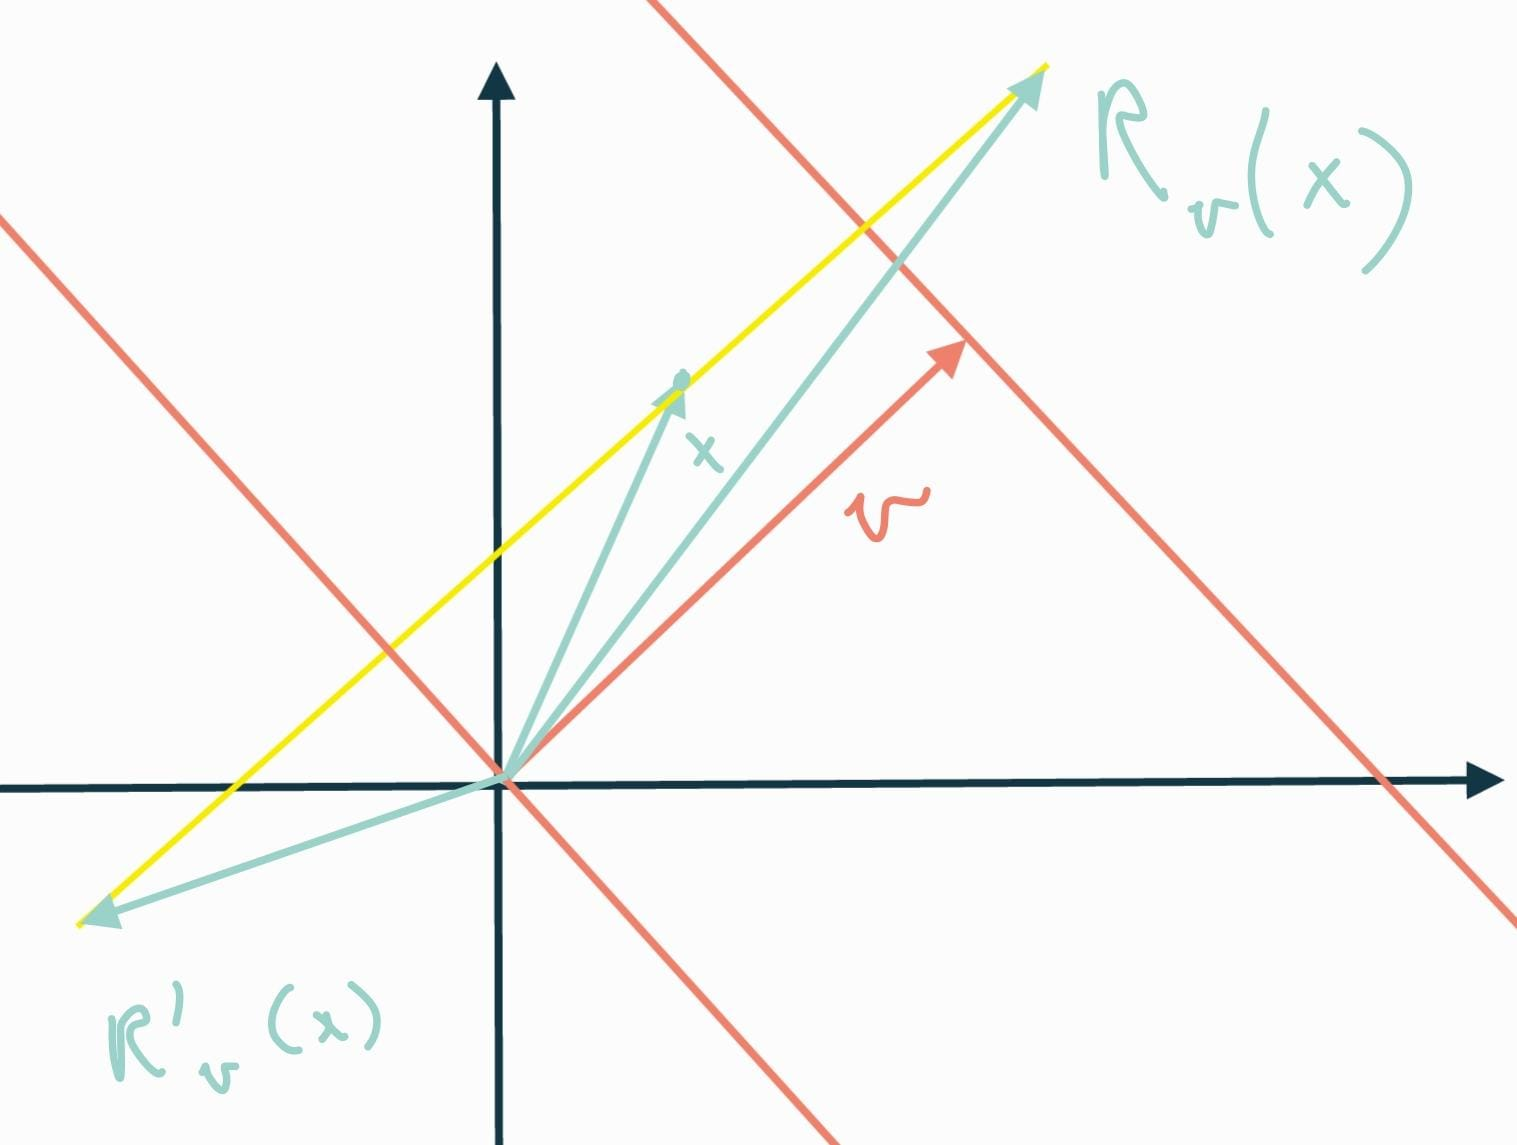
\includegraphics[width=.8\textwidth]{reflections}
\end{figure}

\begin{lemma}
Let $\Cl(V,q)$ be a Clifford algebra and $\vec{v}, \vec{w}, \vec{x}\in V$ be vectors. Then
\begin{enumerate}
\item $\begin{aligned}[t]\big(R_{\vec{v}}\circ R_{\vec{w}}\big)(\vec{x}) &= 2 \vec{v} - 2\vec{v}^{-1}\vec{w}\vec{v} + (\vec{w}\vec{v})^{-1}\vec{x}(\vec{w}\vec{v}) \\
&= 2 \vec{v} - 2 \vec{w} - 4 \frac{\vec{v}\cdot \vec{w}}{\vec{v}^2}\vec{v} + (\vec{w}\vec{v})^{-1}\vec{x}(\vec{w}\vec{v});\end{aligned}$
\item $R_{\vec{v}}\circ R_{\vec{v}} = \id_V$;
\item $\big(R_{\vec{v}}\circ R_{\vec{v}/2}\big)(\vec{x}) = \vec{v} + \vec{x}$;
\item $R_{\vec{v}}' = R_{\vec{v}}\circ R_{2\vec{v}}\circ R_{\vec{v}}$.
\end{enumerate}
\end{lemma}
So translations and reflections about hyperplanes through the origin can be expressed as compositions of reflections about affine hyperplanes.
\begin{proof}
(1) We calculate
\begin{align*}
\big(R_{\vec{v}}\circ R_{\vec{w}}\big)(\vec{x}) &= 2 \vec{v} - \vec{v}^{-1}\big(2 \vec{w} - \vec{w}^{-1} \vec{x}\vec{w}\big)\vec{v} \\
&= 2 \vec{v} - 2\vec{v}^{-1}\vec{w}\vec{v} + (\vec{w}\vec{v})^{-1}\vec{x}(\vec{w}\vec{v}).
\end{align*}

(2) We calculate, using (1),
\begin{align*}
\big(R_{\vec{v}}\circ R_{\vec{v}}\big)(\vec{x}) &= 2 \vec{v} - 2\vec{v}^{-1} \vec{v} \vec{v} + (\vec{v}\vec{v})^{-1}\vec{x}(\vec{v}\vec{v}) \\
&= 2 \vec{v} - 2 \vec{v} + \vec{x} = \vec{x}.
\end{align*}

(3) From (1) we have
\begin{align*}
\big(R_{\vec{v}}\circ R_{\vec{v}/2}\big)(\vec{x}) &= 2 \vec{v} - 2(\vec{v})^{-1}\frac{\vec{v}}{2}(\vec{v}) + (\vec{v}\frac{\vec{v}}{2})^{-1}\vec{x}(\frac{\vec{v}}{2}\vec{v}) \\
&= 2 \vec{v} - \vec{v} + \vec{x} \\
&= \vec{v} + \vec{x}.
\end{align*}

(4) We calculate, using (3),
\begin{align*}
\big(R_{\vec{v}} \circ R_{2\vec{v}}\circ R_{\vec{v}}\big)(\vec{x}) &= R_{\vec{v}}\big(2 \vec{v} + \vec{x}\big) \\
&= 2 \vec{v}-\vec{v}^{-1}\big(2 \vec{v} + \vec{x}\big)\vec{v} \\
&= 2 \vec{v} - 2 \vec{v} - \vec{v}^{-1}\vec{x}\vec{v} \\
&= - \vec{v}^{-1}\vec{x}\vec{v} \\
&= R_{\vec{v}}'(\vec{x})
\end{align*}
\end{proof}

\begin{figure}[h!]
\centering
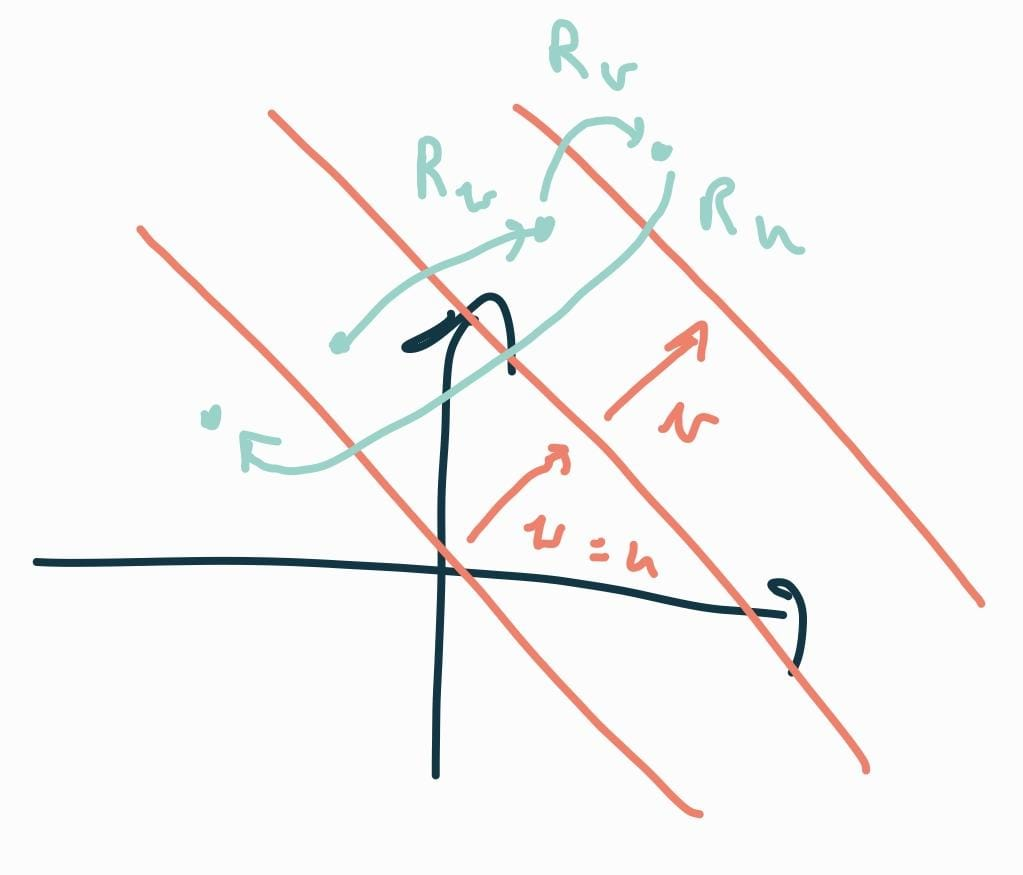
\includegraphics[width=.8\textwidth]{reflectionAboutHyperplaneThroughOrigin}
\caption{Reflection about hyperplane through origin can be expressed as the composition of two normal reflections.}
\end{figure}


\begin{lemma}
Let $\Cl(V,q)$ be a Clifford algebra and $\vec{v}, \vec{x}\in V$. Then $R_{\vec{v}}(\vec{x}) = 2 P_{\vec{v}}(\vec{x}) - \vec{x}$.
\end{lemma}
\begin{proof}
We calculate
\begin{align*}
2 P_{\vec{v}}(\vec{x}) - \vec{x} &= 2 \big(\vec{v}+ (\vec{x}\wedge \vec{v})\vec{v}^{-1}\big) - \vec{x} \\
&= 2\vec{v}+ (\vec{x}\vec{v}- \vec{v}\vec{x})\vec{v}^{-1} - \vec{x} \\
&= 2\vec{v}+ \vec{x}- \vec{v}\vec{x}\vec{v}^{-1} - \vec{x} \\
&= 2\vec{v}+ - \vec{v}^{-1}\vec{x}\vec{v} \\
&= R_{\vec{v}}(\vec{x}).
\end{align*}
\end{proof}

\subsubsection{Rotations}
\begin{figure}[h!]
\centering
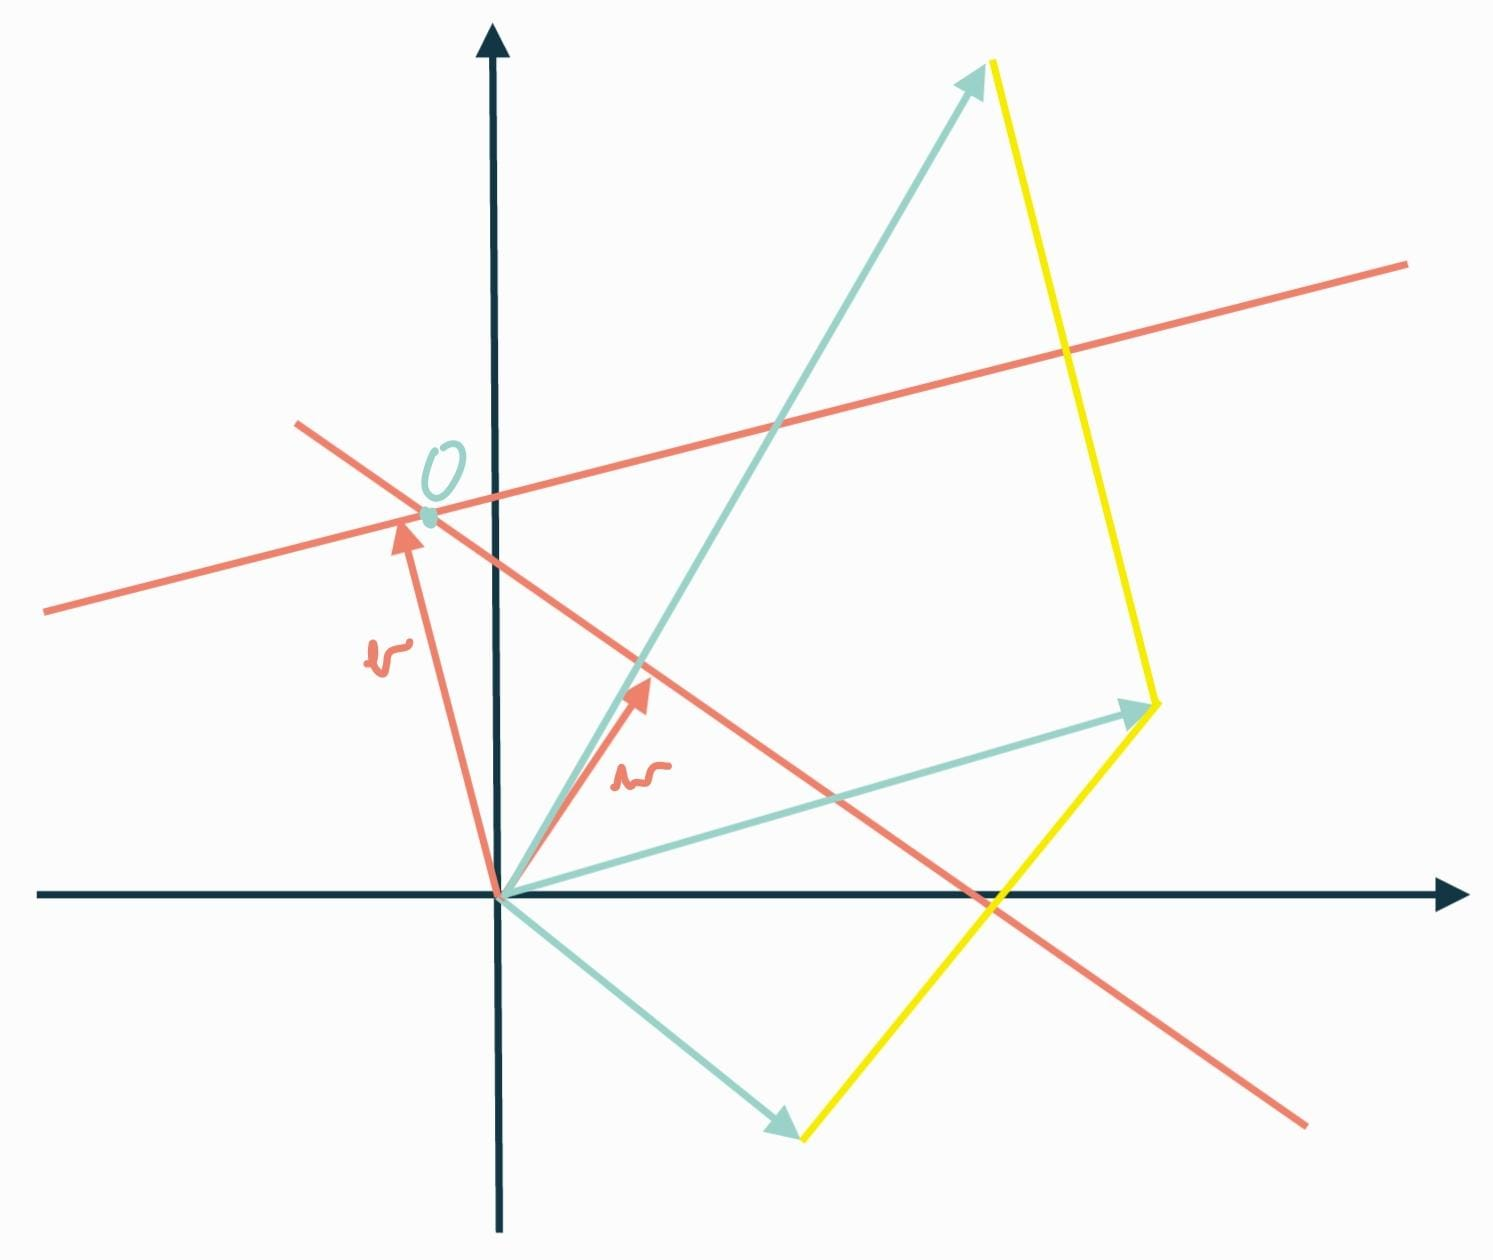
\includegraphics[width=.8\textwidth]{doubleReflection}
\caption{Rotation as double reflection.}
\end{figure}

\begin{figure}[h!]
\centering
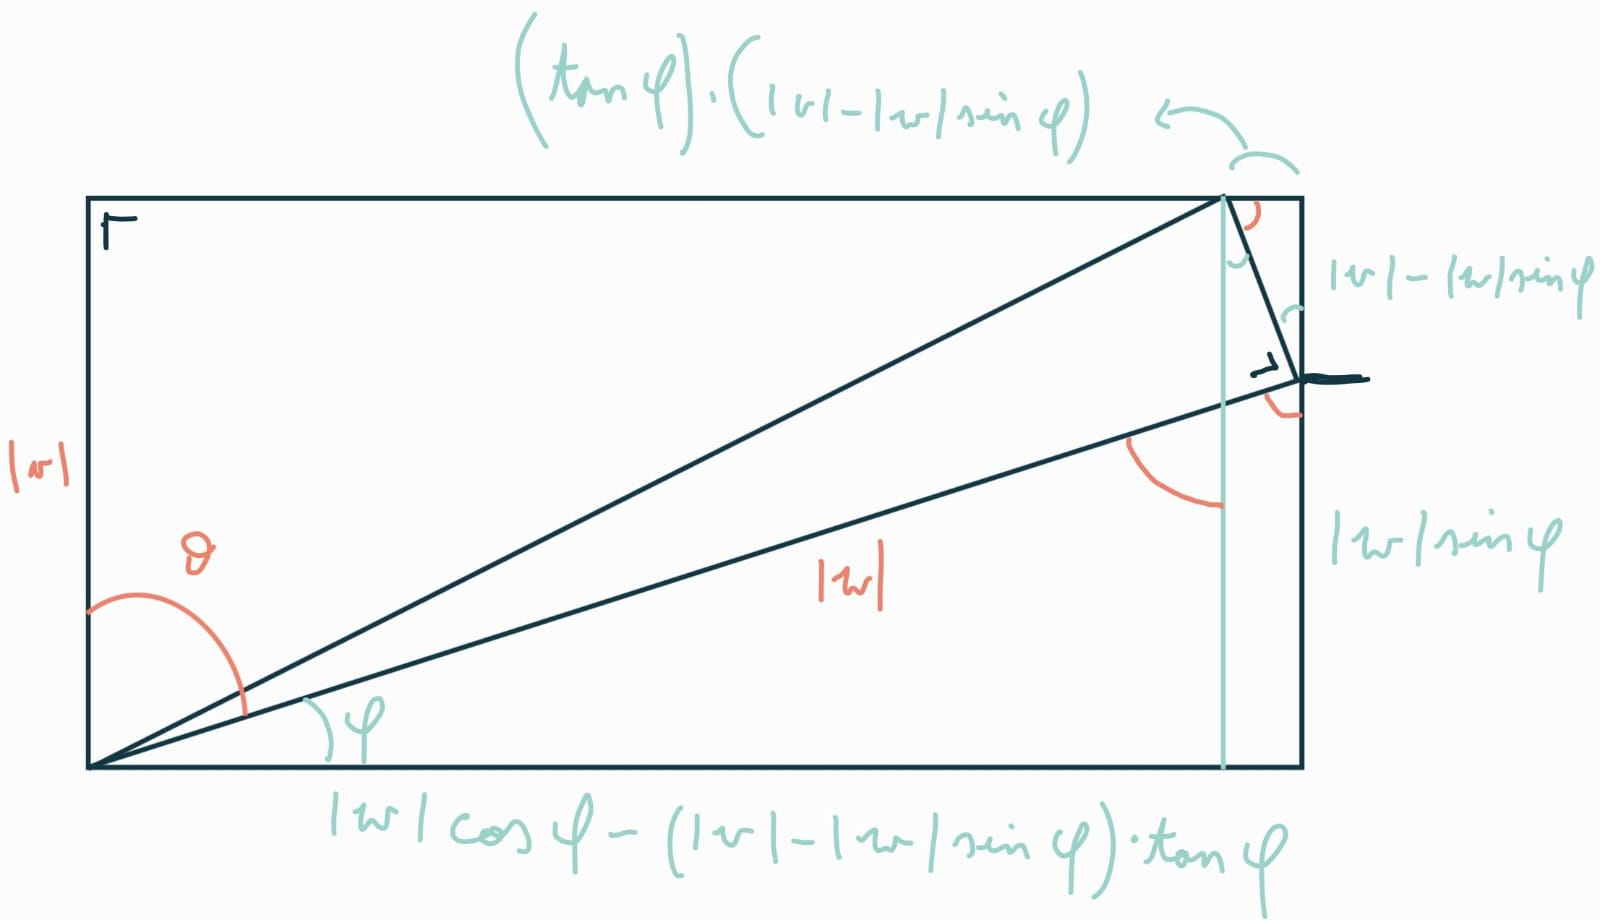
\includegraphics[width=.8\textwidth]{centreOfRotationConstruction}
\caption{Construction of the centre of rotation} 
\end{figure}

\begin{note}
Let $\vec{e}$ be the unit vector in the direction of $\vec{w}_{\perp\vec{v}}$. Then
\begin{align*}
\vec{v} + \big(|\vec{w}|\cos\varphi - |\vec{v}|\tan\varphi + |\vec{w}|\sin\varphi\tan\varphi\big)\vec{e} &= \vec{v} + \big(|\vec{w}|\sin\theta - |\vec{v}|\cot\theta + |\vec{w}|\frac{\cos^2\theta}{\sin\theta}\big)\vec{e} \\
&= \vec{v} + \vec{w}_{\perp\vec{v}} - \frac{\vec{v}\cdot \vec{w}}{|\vec{w}|\sin\theta}\vec{e} + \frac{|\vec{v}|^2|\vec{w}|^2\cos^2\theta}{|\vec{v}|^2 |\vec{w}|\sin\theta}\vec{e} \\
&= \vec{v} + \vec{w}_{\perp\vec{v}} - (\vec{v}\cdot \vec{w})\vec{w}_{\perp\vec{v}}^{-1} + \frac{(\vec{v}\cdot \vec{w})^2}{|\vec{v}|^2 }\vec{w}_{\perp\vec{v}}^{-1} \\
&= \vec{v} + \vec{w}_{\perp\vec{v}}  + \Big(\frac{\vec{v}\cdot \vec{w}}{\vec{v}^2} - 1\Big)(\vec{v}\cdot \vec{w})\vec{w}_{\perp\vec{v}}^{-1}.
\end{align*}
Now, using \ref{parallelPerpendicularComponentConstructions}, we can rewrite this as follows:
\begin{align*}
\vec{v} + \vec{w}_{\perp\vec{v}}  + \Big(\frac{\vec{v}\cdot \vec{w}}{\vec{v}^2} - 1\Big)(\vec{v}\cdot \vec{w})\vec{w}_{\perp\vec{v}}^{-1} &= \vec{v} + \Big(\vec{w} - \frac{\vec{w}\cdot \vec{v}}{\vec{v}^2}\vec{v}\Big) + \Big(\frac{\vec{v}\cdot \vec{w}}{\vec{v}^2} - 1\Big)(\vec{v}\cdot \vec{w})\frac{\vec{v}^2 \vec{w} - (\vec{w}\cdot \vec{v})\vec{v}}{\vec{w}^2 \vec{v}^2 - (\vec{w}\cdot \vec{v})^2} \\
&= \vec{v} + \Big(\vec{w} - \frac{\vec{w}\cdot \vec{v}}{\vec{v}^2}\vec{v}\Big) + \big(\vec{v}\cdot \vec{w} - \vec{v}^2\big)(\vec{v}\cdot \vec{w})\frac{\vec{v}^2 \vec{w} - (\vec{w}\cdot \vec{v})\vec{v}}{\vec{v}^2\big(\vec{w}^2 \vec{v}^2 - (\vec{w}\cdot \vec{v})^2\big)} \\
&= \Big(1 + \frac{(\vec{v}\cdot \vec{w} - \vec{v}^2)(\vec{v}\cdot \vec{w})\cancel{\vec{v}^2}}{\cancel{\vec{v}^2}\big(\vec{w}^2 \vec{v}^2 - (\vec{w}\cdot \vec{v})^2\big)}\Big) \vec{w} + \Big(1 - \frac{\vec{w}\cdot \vec{v}}{\vec{v}^2} - \frac{(\vec{v}\cdot \vec{w} - \vec{v}^2)(\vec{v}\cdot \vec{w})^2}{\vec{v}^2\big(\vec{w}^2 \vec{v}^2 - (\vec{w}\cdot \vec{v})^2\big)}\Big)\vec{v}
\end{align*}
We consider the scalar factor in front of the $\vec{w}$:
\begin{align*}
1 + \frac{(\vec{v}\cdot \vec{w} - \vec{v}^2)(\vec{v}\cdot \vec{w})}{\vec{w}^2 \vec{v}^2 - (\vec{w}\cdot \vec{v})^2} &= 1 + \frac{(\vec{v}\cdot \vec{w})^2 - (\vec{v}\cdot \vec{w})\vec{v}^2}{\vec{w}^2 \vec{v}^2 - (\vec{w}\cdot \vec{v})^2} \\
&= \frac{\vec{w}^2 \vec{v}^2 - \cancel{(\vec{w}\cdot \vec{v})^2} + \cancel{(\vec{v}\cdot \vec{w})^2} - (\vec{v}\cdot \vec{w})\vec{v}^2}{\vec{w}^2 \vec{v}^2 - (\vec{w}\cdot \vec{v})^2} \\
&= \frac{\big(\vec{w}^2 - (\vec{v}\cdot \vec{w})\big)\vec{v}^2}{\vec{w}^2 \vec{v}^2 - (\vec{w}\cdot \vec{v})^2}.
\end{align*}
We now consider the scalar factor in front of the $\vec{v}$:
\begin{align*}
1 - \frac{\vec{w}\cdot \vec{v}}{\vec{v}^2} - \frac{(\vec{v}\cdot \vec{w} - \vec{v}^2)(\vec{v}\cdot \vec{w})^2}{\vec{v}^2\big(\vec{w}^2 \vec{v}^2 - (\vec{w}\cdot \vec{v})^2\big)} &= \frac{\vec{v}^4 \vec{w}^2 - \cancel{(\vec{v}\cdot \vec{w})^2 \vec{v}^2} - \vec{v}^2 \vec{w}^2 (\vec{v}\cdot \vec{w}) + \bcancel{(\vec{v}\cdot \vec{w})^3} - \bcancel{(\vec{v}\cdot \vec{w})^3} + \cancel{\vec{v}^2(\vec{v}\cdot \vec{w})^2}}{\vec{v}^2\big(\vec{w}^2 \vec{v}^2 - (\vec{w}\cdot \vec{v})^2\big)} \\
&= \frac{\vec{v}^4 \vec{w}^2 - \vec{v}^2 \vec{w}^2 (\vec{v}\cdot \vec{w})}{\vec{v}^2\big(\vec{w}^2 \vec{v}^2 - (\vec{w}\cdot \vec{v})^2\big)} \\
&= \frac{\big(\vec{v}^2 - (\vec{v}\cdot \vec{w})\big)\vec{w}^2}{\vec{w}^2 \vec{v}^2 - (\vec{w}\cdot \vec{v})^2}.
\end{align*}
The whole vector is then
\[ \frac{\big(\vec{v}^2 - (\vec{v}\cdot \vec{w})\big)\vec{w}^2}{\vec{w}^2 \vec{v}^2 - (\vec{w}\cdot \vec{v})^2}\vec{v} + \frac{\big(\vec{w}^2 - (\vec{v}\cdot \vec{w})\big)\vec{v}^2}{\vec{w}^2 \vec{v}^2 - (\vec{w}\cdot \vec{v})^2}\vec{w}. \]
Note that it is unchanged if we exchange $\vec{v}$ and $\vec{w}$.
\end{note}

\begin{lemma}
Let $\Cl(V,q)$ be a Clifford algebra and $\vec{v}, \vec{w}\in V$. Then the vector
\[ \vec{u} \defeq \frac{\big(\vec{v}^2 - (\vec{v}\cdot \vec{w})\big)\vec{w}^2}{\vec{w}^2 \vec{v}^2 - (\vec{w}\cdot \vec{v})^2}\vec{v} + \frac{\big(\vec{w}^2 - (\vec{v}\cdot \vec{w})\big)\vec{v}^2}{\vec{w}^2 \vec{v}^2 - (\vec{w}\cdot \vec{v})^2}\vec{w} \]
is a fixed point of $R_{\vec{v}}\circ R_{\vec{w}}$.
\end{lemma}
\begin{proof}
It is enough to prove that it is a fixed point of both $R_{\vec{v}}$ and $R_{\vec{w}}$. For the first part, we need to show $\vec{u} = R_{\vec{v}}(\vec{u}) = 2 \vec{v} - \vec{v}^{-1}\vec{u}\vec{v}$.
We calculate
\begin{align*}
2 \vec{v} - \vec{v}^{-1} \vec{u}\vec{v} &= 2 \vec{v} - \frac{\big(\vec{v}^2 - (\vec{v}\cdot \vec{w})\big)\vec{w}^2}{\vec{w}^2 \vec{v}^2 - (\vec{w}\cdot \vec{v})^2}\vec{v}^{-1}\vec{v}\vec{v} - \frac{\big(\vec{w}^2 - (\vec{v}\cdot \vec{w})\big)\vec{v}^2}{\vec{w}^2 \vec{v}^2 - (\vec{w}\cdot \vec{v})^2}\vec{v}^{-1} \vec{w}\vec{v} \\
&= 2 \vec{v} - \frac{\big(\vec{v}^2 - (\vec{v}\cdot \vec{w})\big)\vec{w}^2}{\vec{w}^2 \vec{v}^2 - (\vec{w}\cdot \vec{v})^2}\vec{v} - \frac{\big(\vec{w}^2 - (\vec{v}\cdot \vec{w})\big)\vec{v}^2}{\vec{w}^2 \vec{v}^2 - (\vec{w}\cdot \vec{v})^2}\Big(2 \frac{\vec{v}\cdot \vec{w}}{\vec{v}^2}\vec{v} - \vec{w}\Big) \\
&= \Big(2 - \frac{\big(\vec{v}^2 - (\vec{v}\cdot \vec{w})\big)\vec{w}^2}{\vec{w}^2 \vec{v}^2 - (\vec{w}\cdot \vec{v})^2} - \frac{\big(\vec{w}^2 - (\vec{v}\cdot \vec{w})\big)\vec{v}^2}{\vec{w}^2 \vec{v}^2 - (\vec{w}\cdot \vec{v})^2}2 \frac{\vec{v}\cdot \vec{w}}{\vec{v}^2}\Big)\vec{v} + \frac{\big(\vec{w}^2 - (\vec{v}\cdot \vec{w})\big)\vec{v}^2}{\vec{w}^2 \vec{v}^2 - (\vec{w}\cdot \vec{v})^2}\vec{w} \\
&= \frac{\cancel{2} \vec{v}^4 \vec{w}^2 - \bcancel{2 \vec{v}^2 (\vec{v}\cdot \vec{w})^2} - \cancel{\vec{v}^4 \vec{w}^2} + \xcancel{\vec{v}^2 \vec{w}^2(\vec{v}\cdot \vec{w})} - \xcancel{2}\vec{v}^2\vec{w}^2(\vec{v}\cdot \vec{w}) + \bcancel{2\vec{v}^2 (\vec{v}\cdot \vec{w})^2}}{\vec{v}^2\big(\vec{v}^2 \vec{w}^2 - (\vec{v}\cdot \vec{w})^2\big)}\vec{v} + \frac{\big(\vec{w}^2 - (\vec{v}\cdot \vec{w})\big)\vec{v}^2}{\vec{w}^2 \vec{v}^2 - (\vec{w}\cdot \vec{v})^2}\vec{w} \\
&= \frac{\vec{v}^4 \vec{w}^2 - \vec{v}^2\vec{w}^2(\vec{v}\cdot \vec{w})}{\vec{v}^2\big(\vec{v}^2 \vec{w}^2 - (\vec{v}\cdot \vec{w})^2\big)}\vec{v} + \frac{\big(\vec{w}^2 - (\vec{v}\cdot \vec{w})\big)\vec{v}^2}{\vec{w}^2 \vec{v}^2 - (\vec{w}\cdot \vec{v})^2}\vec{w} \\
&= \frac{\big(\vec{v}^2 - (\vec{v}\cdot \vec{w})\big)\vec{w}^2}{\vec{v}^2 \vec{w}^2 - (\vec{v}\cdot \vec{w})^2}\vec{v} + \frac{\big(\vec{w}^2 - (\vec{v}\cdot \vec{w})\big)\vec{v}^2}{\vec{w}^2 \vec{v}^2 - (\vec{w}\cdot \vec{v})^2}\vec{w} = \vec{u}.
\end{align*}
The claim for $R_{\vec{w}}$ follows similarly, since $\vec{u}$ is unchanged under exchange of $\vec{v}$ and $\vec{w}$.
\end{proof}


\begin{proposition}
Let $\Cl(V,q)$ be a Clifford algebra and $\vec{v}, \vec{w}\in V$. Then
\end{proposition}



\subsubsection{Rotors and rotations}
\url{https://marctenbosch.com/quaternions/#h_16}
-> why composition of rotors works.

\begin{proposition}
$e^{\theta} \leftrightarrow \vhat{a}\vhat{b}$
\end{proposition}

\begin{lemma}
Let $\vhat{u}, \vhat{v}$ be unit vectors in a geometric algebra $\G^n$ and let $\{\vec{e}_1, \vec{e}_2\}$ be an orthonormal basis of $\Span\{\vhat{u},\vhat{v}\}$. Then
\[ \vhat{v}\vhat{u} = \cos\theta + \sin\theta \vhat{e}_1\vhat{e}_2 = e^{\theta \vhat{e}_1\vhat{e}_2}, \]
for some $\theta \in [ 0,2\pi ]$.
\end{lemma}
\begin{proof}
TODO
\end{proof}


In the plane $\Span\{\vhat{e}_1,\vhat{e}_2\}$, a rotation that maps $\vhat{u}$ to $\vhat{v}$ should act as $\lambda_{\vhat{v}\vhat{u}}$. On vectors perpendicular to the plane it should act as the identity.


\begin{proposition}
Let $\vhat{u}, \vhat{v}$ be unit vectors in a geometric algebra $\G^n$ and let $\{\vec{e}_1, \vec{e}_2\}$ be an orthonormal basis of $\Span\{\vhat{u},\vhat{v}\}$. Set $\vec{i} \defeq \vec{e}_1\wedge \vec{e}_2 = \vec{e}_1\vec{e}_2$. Then the rotation $R_{\vhat{v}\from\vhat{u}}$ that maps $\vhat{u}$ to $\vhat{v}$ can be written as
\[ R_{\vhat{v}\from\vhat{u}}: V \to V: \vec{w} \mapsto e^{\vec{i}\theta/2}\vec{w}e^{-\vec{i}\theta/2}. \]
Thus $R_{\vhat{v}\from\vhat{u}} = \Ad_{e^{\vec{i}\theta/2}} = \widetilde{\Ad}_{e^{\vec{i}\theta/2}}$.
\end{proposition}
\begin{proof}
We write $\vec{w} = \vec{w}_\parallel + \vec{w}_\perp \in \Span\{\vhat{u},\vhat{v}\} \oplus \Span\{\vhat{u},\vhat{v}\}^\perp$.
Then
\begin{align*}
R_{\vhat{v}\from\vhat{u}}(\vec{w}) &= e^{\vec{i}\theta}\vec{w}_\parallel + \vec{w}_\perp \\
&= e^{\vec{i}\theta/2}e^{\vec{i}\theta/2}\vec{w}_\parallel + e^{\vec{i}\theta/2}e^{-\vec{i}\theta/2}\vec{w}_\perp \\
&= e^{\vec{i}\theta/2}\vec{w}_\parallel e^{-\vec{i}\theta/2} + e^{\vec{i}\theta/2}\vec{w}_\perp e^{-\vec{i}\theta/2} \\
&= e^{\vec{i}\theta/2}(\vec{w}_\parallel + \vec{w}_\perp) e^{-\vec{i}\theta/2} = e^{\vec{i}\theta/2}\vec{w} e^{-\vec{i}\theta/2}.
\end{align*}
We have used that elements of $\Span\{\vhat{u},\vhat{v}\}$ commute with $\vec{i}$ and elements of $\Span\{\vhat{u},\vhat{v}\}^\perp$ anticommute with $\vec{i}$.
\end{proof}
\begin{corollary}
Let $\vhat{n}$ be a unit vector in $\G^3$ and $\vec{I}$ a unit pseudoscalar. Then a rotation of $\theta$ radians around $\vhat{n}$ is given by
\[ R_{\vhat{n},\theta}: V \to V: \vec{w} \mapsto e^{\vec{n}\vec{I}\theta/2}\vec{w}e^{-\vec{n}\vec{I}\theta/2}. \]
Thus $R_{\vhat{n},\theta} = \Ad_{e^{\vec{n}\vec{I}\theta/2}} = \widetilde{\Ad}_{e^{\vec{n}\vec{I}\theta/2}}$. The direction is determined by the orientation of $\vec{I}$.
\end{corollary}
\begin{proof}
TODO
\end{proof}

\begin{definition}
We call an element of $\G^n$ of the form $e^{\vec{i}\theta/2}$ a \udef{rotor}.
\end{definition}

TODO $\Spin^+$!

\section{Representations}

\begin{definition}
Let $K \subseteq k$ be fields, $V$ a vector space over $k$ and $q$ a quadratic form on $V$. Then a \udef{$K$-representation} of the Clifford algebra $\Cl(V,q)$ is a $k$-algebra homomorphism
\[ \rho: \Cl(V,q) \to \Hom_K(W,W) \]
where $W$ is a finite dimensional vector space over $K$. The space $W$ is then a \udef{$\Cl(V,q)$-module} over $K$.
\end{definition}

Usually we will take the field $K$ to be $\R,\C,\mathbb{H}$.

\begin{lemma}
\begin{enumerate}
\item A complex representation of $\Cl_{r,s}$ automatically extends to a representation of
\[ \Cl_{r,s}\otimes_\R \C \cong \cCl_{r+s}. \]
\item A quaternionic representation of $\Cl_{r,s}$ is automatically complex.
\end{enumerate}
\end{lemma}

\section{Lie algebra structures}

\begin{proposition}
The Lie subalgebra of $(\Cl_n, [\cdot,\cdot])$ corresponding to the subgroup $\Spin_n\subset \Cl_n^\times$ is
\[ \mathfrak{spin}_n = {\textstyle \bigwedge^2}\R^n. \]
In particular, $\bigwedge^2\R^n$ is closed under the bracket operation.
\end{proposition}
\begin{proof}
We are looking for tangent vectors to the submanifold $\Spin_n$ at $\vec{1}$. Fix an orthonormal basis $e_1,\ldots, e_n$ of $\R^n$ and consider the curve
\[ \gamma(t) = (e_i\cos t+ e_j\sin t)(-e_i\cos t+ e_j\sin t) = (\cos^2 t - \sin^2 t)+2e_ie_j\sin t\cos t = \cos(2t)\sin(2t)e_ie_j. \]
This curve lies in $\Spin_n$, satisfies $\gamma(0) = \vec{1}$ and its tangent vector at $\gamma(0)$ is $2e_ie_j$. Hence $\mathfrak{spin}_n$ contains $\Span_\R\{e_ie_j\} = \bigwedge^2\R^n$. Since $\dim_\R(\mathfrak{spin}_n)$
\end{proof}






\section{Geometry and geometric algebra}
\url{http://www.faculty.luther.edu/~macdonal/GAConstruct.pdf}
\subsection{Definitions}

\begin{definition}
A \udef{geometric algebra} $\mathfrak{G}$ is a real unital associative algebra of the form
\[ \mathfrak{G} = \bigoplus_{r\in \N}\mathfrak{G}_r \]
such that
\begin{align*}
\mathfrak{G}_0 &= \Span\{\vec{1}\} \\
\mathfrak{G}_r &= \Span\setbuilder{\vec{a}_1\vec{a}_2\ldots\vec{a}_r}{\vec{a}_1,\ldots,\vec{a}_r \in \mathfrak{G}_1, \; \forall i,j\leq r: \vec{a}_i \vec{a}_j = -\vec{a}_j \vec{a}_i} & \text{for all $r>1$}.
\end{align*}
We also assume that the multiplication satisfies
\[ \forall \vec{a} \in \mathfrak{G}_1: \quad \vec{a}^2 = \vec{a}\vec{a} = \lambda \vec{1} \in \mathfrak{G}_0 \qquad \text{for some $\lambda \in \R^{> 0}$} \]
and that for each element $a$ of $\mathfrak{G}_r\setminus\{0\}$ there exists a vector $\vec{a}\in\mathfrak{G}_1$ such that $\vec{a}a \in \mathfrak{G}_{r+1}\setminus\{0\}$.

We then call
\begin{itemize}
\item $\sqrt{\lambda}$ the \udef{magnitude of $\vec{a}$}, denoted $|\vec{a}|$;
\item the projection $\mathfrak{G} \to \mathfrak{G}_r$ the \udef{grade operator}, denoted $\grade{\cdot}_r$;
\item the multiplication of $\mathfrak{G}$ the \udef{geometric product} on $\mathfrak{G}$;
\item elements of $\mathfrak{G}$ \udef{multivectors};
\item elements of $\mathfrak{G}_r$ \udef{$r$-vectors} or \udef{homogenous multivectors}; in particular $0$-vectors are called \udef{scalars}, $1$-vectors \udef{vectors}, $2$-vectors \udef{bivectors} \ldots
\item $r$-vectors of the form $\vec{a}_1\vec{a}_2\ldots\vec{a}_r$ where $\vec{a}_1,\ldots,\vec{a}_r \in \mathfrak{G}_1$ anti-commute are called \udef{simple $r$-vectors} or \udef{$r$-blades}.
\end{itemize}
We use lowercase letters $a,b,c \ldots$ to denote multivectors, Greek letters $\mu, \nu, \lambda \ldots$ for scalars and bold letters $\vec{u}, \vec{v}, \vec{w} \ldots$ for vectors. Often we will use subscripts to denote the grade of a multivector, e.g\ $a_r$ is an $r$-vector. Capital letters with subscript, e.g\ $A_r$, will be used to denote $r$-blades.
\end{definition}

So for any $a\in \mathfrak{G}$, we can write
\[ a = \grade{a}_0 + \grade{a}_1 + \ldots + \grade{a}_n  = \sum_{r=0}^n \grade{a}_i  \] for some $n\in\N$.

We make the convention that negative grades are always zero.

Because of the assumption that no $\mathfrak{G}_r$ is trivial, we need $\mathfrak{G}_1$ to be infinite-dimensional.


\begin{definition}
Let $\mathfrak{G}$ be a geometric algebra. We define the \udef{reverse} operation $\dagger$ on $\mathfrak{G}$ as the unique linear operation such that
\begin{align*}
\vec{1}^\dagger &= \vec{1} \\
\vec{u}^\dagger &= \vec{u} \qquad \vec{u}\in\mathfrak{G}_1 \\
(\vec{v}_1 \vec{v}_2 \ldots \vec{v}_r)^\dagger &= \vec{v}_r \ldots \vec{v}_2 \vec{v}_1 \qquad \vec{v}_1, \ldots, \vec{v}_r \in \mathfrak{G}_1.
\end{align*}
\end{definition}
Note that we have specified $\dagger$ on all basis elements of $\mathfrak{G}$, so it is well-defined and uniquely determined, cfr. \ref{linearMapsDeterminedByBasis}.

\begin{lemma}
Let $a,b \in \mathfrak{G}$. Then
\begin{enumerate}
\item $(a^\dagger)^\dagger = a$;
\item $(ab)^\dagger = b^\dagger a^\dagger$;
\item $\grade{a^\dagger}_r = \grade{a}_r^\dagger = (-1)^{r(r-1)/2}\grade{a}_r$;
\item $\grade{a}_r = (-1)^{r(r-1)/2}\grade{a}_r^\dagger$;
\item $\grade{a_rb_s}_t = (-1)^{\frac{1}{2}(r(r-1) + s(s-1) + t(t-1))}\grade{b_sa_r}_t$.
\end{enumerate}
\end{lemma}
Notice we are only interested in the exponent of $(-1)$ modulo $2$.

\begin{definition}
Let $\mathfrak{G}$ be a geometric algebra. We define the \udef{inner product} $\cdot$ on homogeneous multivectors by
\[ a_r\cdot b_s = \begin{cases}
0 & \text{$r=0$ or $s=0$} \\
\grade{a_rb_s}_{|r-s|} & \text{else}.
\end{cases}  \]
The inner product is bilinear on homogeneous multivectors and can thus be extended linearly to arbitrary multivectors.
\end{definition}
So for arbitrary multivectors we have
\[ a\cdot b = \sum_r\sum_s \grade{a}_r\cdot \grade{b}_s. \]

\begin{definition}
Let $\mathfrak{G}$ be a geometric algebra. We define the \udef{outer product} $\wedge$ on homogeneous multivectors by
\[ a_r\wedge b_s = \grade{a_rb_s}_{r+s} \]
The outer product is bilinear on homogeneous multivectors and can thus be extended linearly to arbitrary multivectors.
\end{definition}
So for arbitrary multivectors we have
\[ a\wedge b = \sum_r\sum_s \grade{a}_r\wedge \grade{b}_s. \]
For scalars $\lambda \in \mathfrak{G}^0$, we have
\[ a \wedge \lambda = \lambda\wedge a = \lambda a \qquad a \in \mathfrak{G}. \]
We have explicitly excluded this in the inner product.

\begin{lemma}
If $a = \vec{v}_1 \vec{v}_2\ldots \vec{v}_r$, then $a\in \bigoplus_{i\leq r}\mathfrak{G}_i$.

If $a$ is an $r$-blade and $\beta$ an orthogonal basis for $\mathfrak{G}_1$, then there exist $\vec{e}_1,\ldots, \vec{e}_r \in \beta$ such that
\[ a = \lambda \vec{e}_1 \ldots \vec{e}_r \]


 be an $r$-blade, then
\[\vec{v}_1 \vec{v}_2\ldots \vec{v}_r = \vec{v}_1 \wedge \vec{v}_2 \wedge\ldots\wedge \vec{v}_r.\]
\end{lemma}

\begin{note}
We introduce an order of operations (from highest priority to lowest):
\begin{enumerate}
\item outer product;
\item inner product;
\item geometric product.
\end{enumerate}
\end{note}

\begin{lemma}
Let $a_r,b_s$ be homogeneous vectors in $\mathfrak{G}$. Then
\begin{enumerate}
\item $a_r\cdot b_s = (-1)^{s(r-1)}b_s\cdot a_r$ for $r\geq s$;
\item $a_r \wedge b_s = (-1)^{rs}b_s \wedge a_r$.
\end{enumerate}
\end{lemma}
\begin{proof}
(1) We calculate
\[ a_r\cdot b_s = \grade{a_rb_s}_{|r-s|} = (-1)^{\frac{1}{2}(r(r-1) + s(s-1) + |r-s|(|r-s|-1))}\grade{a_rb_s}_{|r-s|}. \]
We can simplify the exponent, assuming $r\geq s$, to
\[ r^2 + s^2 -r -sr \equiv r+s+r+sr \equiv s+sr \equiv sr-s \mod 2.\]
(2) We calculate
\[ a_r \wedge b_s = \grade{a_rb_s}_{r+s} = (-1)^{\frac{1}{2}(r(r-1) + s(s-1) + (r+s)((r+s)-1))}\grade{a_rb_s}_{r+s}. \]
We can simplify the exponent to
\[ r^2 -r+s^2 -s + rs \equiv r-r+s-s+rs \equiv rs \mod 2. \]
\end{proof}

By the fact that the definitions of inner and outer product make sense it is obvious that the geometric product does not preserve grade, or even homogeneity. It does, however, preserve a $\Z_2$-grading: we can split
\[ \mathfrak{G} = \mathfrak{G}_\text{even} \oplus \mathfrak{G}_\text{odd} \qquad \text{where}\quad \begin{cases}
\mathfrak{G}_\text{even} \defeq \bigoplus_{r\in \N}\mathfrak{G}_{2r} \\
\mathfrak{G}_\text{odd}\; \defeq \bigoplus_{r\in \N}\mathfrak{G}_{2r+1}.
\end{cases} \]
We have the linear projection operators $\grade{\cdot}_+:\mathfrak{G}\to \mathfrak{G}_\text{even}$ and $\grade{\cdot}_-:\mathfrak{G}\to \mathfrak{G}_\text{odd}$. We also write $\mathfrak{G}_+$ instead of $\mathfrak{G}_\text{even}$ and $\mathfrak{G}_-$ instead of $\mathfrak{G}_\text{odd}$.
\begin{proposition}
Let $\mathfrak{G} = \mathfrak{G}_\text{+} \oplus \mathfrak{G}_\text{-}$ be a geometric algebra and let $p,q\in\{+,-\}\cong \Z_2$. Then
\[ \mathfrak{G}_p\mathfrak{G}_q \subset \mathfrak{G}_{pq}. \]
\end{proposition}
\begin{proof}
The grading operators $\grade{\cdot}_\pm$ are linear maps and thus determined by their action on basis elements. Thus it is enough to show that
\[ \grade{A_rB_s}_+ =  \begin{cases}
A_rB_s & (r+s \equiv 0 \mod 2) \\
0 & (r+s \equiv 1 \mod 2)
\end{cases} \qquad \grade{A_rB_s}_- =  \begin{cases}
0 & (r+s \equiv 0 \mod 2) \\
A_rB_s & (r+s \equiv 1 \mod 2)
\end{cases} \]
for any $r$-blade $A_r$ and $s$-blade $B_s$. In fact by associativity of the geometric product, it is enough to show
\[ \vec{v}A_r \]
\end{proof}

\begin{lemma}
Let $\vec{u}, \vec{v} \in \mathfrak{G}_1$. Then
\[ \vec{u}\cdot \vec{v} = \grade{\vec{u}\vec{v}}_0 = \frac{1}{2}(\vec{u}\vec{v} + \vec{v}\vec{u}). \]
\end{lemma}
\begin{proof}
We start from $(\vec{u}+\vec{v})^2 = \vec{u}^2 + \vec{u}\vec{v} + \vec{v}\vec{u} + \vec{v}^2$ and rearrange to get
\[ \vec{u}\vec{v} + \vec{v}\vec{u} = (\vec{u}+\vec{v})^2 - \vec{u}^2 - \vec{v}^2 = |\vec{u}+\vec{v}|^2 - |\vec{u}|^2 - |\vec{v}|^2  \]
which is scalar. Since $\grade{\vec{u}\vec{v}}_0 = \grade{\vec{v}\vec{u}}_0$, we have
\[ \frac{1}{2}(\vec{u}\vec{v} + \vec{v}\vec{u}) = \frac{1}{2}\grade{\vec{u}\vec{v} + \vec{v}\vec{u}}_0 = \grade{\vec{u}\vec{v}}_0 = \vec{u}\cdot \vec{v}. \]
\end{proof}
\begin{corollary}
The geometric inner product restricted to $\mathfrak{G}_1$ is bilinear, symmetric and positive definite. It is thus an inner product as previously defined.
\end{corollary}
The associated definitions are thus also applicable here. In particular two vectors $\vec{u},\vec{v}$ are called \udef{orthogonal} if $\vec{u}\cdot \vec{v} = 0$. By the lemma this is the case when $\vec{u}\vec{v} = - \vec{v}\vec{u}$. This means that the $r$ vectors making up $r$-blades are linearly independent, \ref{orthogonalLinearlyIndependent}.




\begin{lemma}
For any algebra satisfying the other axioms, the direct sum $\mathfrak{G} = \bigoplus_{r\in\N}\mathfrak{G}_r$ is well-defined.
\end{lemma}
\begin{proof}
We need to show that for all $r>s\in \N$, we have $\mathfrak{G}_r\cap\mathfrak{G}_s = \{0\}$. Assume, towards a contradiction, that here exist $a_r,b_s$ such that $a_r = b_s$. Then both $a_r$ and $b_s$ can be written as sums of blades. Now let $D$ be the set of all vectors featured in a blade in this sum. By Gram-Schmidt, we can find an orthogonal basis for $D$ and rewrite $a_r$ and $b_s$ in this basis. As $r>s$, we can find elements of this orthogonal basis to multiply $a_r$ with such that it becomes zero, but $b_s$ remains non-zero (unless it already was zero). TODO: improve proof.
\end{proof}


\begin{lemma}
Let $\vec{u}, \vec{v}_1,\ldots, \vec{v}_n$ be vectors in $\mathfrak{G}_1$. Then
\[ \vec{u}\cdot (\vec{v}_1 \vec{v}_2 \ldots \vec{v}_n) = \sum_{i=1}^n (-1)^{k+1}(\vec{u}\cdot \vec{v}_i)\vec{v}_1\ldots\breve{\vec{v}}_i\ldots \vec{v}_n, \]
where the breve indicates the vector under it is omitted from the product.
\end{lemma}
\begin{proof}

\end{proof}

\begin{lemma}
\[ \vec{u}a_r = \vec{u}\cdot a_r + \vec{u}\wedge a_r = \grade{\vec{u}a_r}_{r-1} + \grade{\vec{u}a_r}_{r+1}. \]
\end{lemma}

\begin{proposition}
Let $\vec{v}\in\mathfrak{G}_1$ and $a_r\in\mathfrak{G}_r$. Then

\end{proposition}





\begin{lemma}
The outer product is associative:
\[ a\wedge(b\wedge c) = (a\wedge b)\wedge c \]
The inner product is not associative, but homogeneous multivectors obey
\begin{align*}
a_r\cdot(b_s \cdot c_t) &= (a_r\wedge b_s)\cdot c_t & &\text{for $r+s\leq t$ and $r,s>0$} \\
a_r\cdot(b_s \cdot c_t) &= (a_r\cdot b_s)\cdot c_t & &\text{for $r+t\leq s$}
\end{align*}
\end{lemma}

\begin{lemma}
\[ \vec{u}\wedge a\wedge \vec{v}\wedge b = -\vec{v}\wedge a\wedge \vec{u}\wedge b  \]
\end{lemma}
$\vec{v}\wedge a \wedge \vec{v} \wedge b = 0$

\subsection{Affine spaces}
\subsection{Projections on 1D spaces}
\[ \sin(\theta) = \norm{a_\perp}/ \norm{a} \qquad \cos(\theta) = \norm{a_\parallel}/\norm{a}. \]
\subsection{The geometric product}

\subsection{Hodge duality}
\subsection{Cross product and triple product}
Cross product not associative

Triple product nice way to find normal vectors with specific orientation.

